\documentclass[aspectratio=169]{beamer}
% Shared preamble for ml/ slide decks.
% Each lecture .tex starts with:
%   \documentclass[aspectratio=169]{beamer}
%   % Shared preamble for ml/ slide decks.
% Each lecture .tex starts with:
%   \documentclass[aspectratio=169]{beamer}
%   % Shared preamble for ml/ slide decks.
% Each lecture .tex starts with:
%   \documentclass[aspectratio=169]{beamer}
%   \input{../preamble}
% Compile from inside the chapter folder so \input{../preamble} resolves.

\usetheme{default}
\usecolortheme{dove}

\setbeamertemplate{navigation symbols}{}
\setbeamertemplate{footline}{%
  \hfill{\large\insertframenumber\,/\,\inserttotalframenumber}\hspace{0.8em}\vspace{0.5em}%
}

% Project palette (existing, kept for backwards compatibility with deferred/*)
\definecolor{popblue}{RGB}{52, 101, 164}
\definecolor{sampred}{RGB}{204, 0, 0}
\definecolor{paramgreen}{RGB}{0, 140, 70}
\definecolor{warnred}{RGB}{180, 40, 40}
\definecolor{orange1}{RGB}{220, 120, 0}
\definecolor{violet1}{RGB}{120, 50, 160}
\definecolor{lightbg}{RGB}{245, 245, 250}

% Armenian flag palette (use these for any 3-color highlight; per CLAUDE.md).
% "Nice versions": slightly de-saturated from the official spec for slide use,
% so they don't burn out under projector colors. Originals kept as *_pure.
\definecolor{armred}{RGB}{200, 30, 40}      % nice red (official #D90012 muted)
\definecolor{armblue}{RGB}{30, 70, 160}     % nice blue (official #0033A0 muted)
\definecolor{armorange}{RGB}{230, 160, 30}  % nice orange (official #F2A800 muted)
\definecolor{armred_pure}{HTML}{D90012}     % official Armenian flag red
\definecolor{armblue_pure}{HTML}{0033A0}    % official Armenian flag blue
\definecolor{armorange_pure}{HTML}{F2A800}  % official Armenian flag orange

\setbeamercolor{frametitle}{fg=popblue}
\setbeamercolor{title}{fg=popblue}

\usepackage{pgfplots}
\usepackage{tikz}
\usetikzlibrary{shapes, arrows.meta, positioning, calc, decorations.pathreplacing, patterns, matrix}
\pgfplotsset{compat=1.18}
\usepackage{amsmath, amssymb, amsfonts}
\usepackage{bm}
\usepackage{dsfont}
\usepackage{array}
\usepackage{pifont}
\usepackage{colortbl}
\usepackage{fontenc}

% Callout boxes. Purely additive - existing decks are unaffected.
% Usage: \begin{tcolorbox}[colback=armblue!8, colframe=armblue, boxrule=0.6pt, arc=2pt,
%                          title=\textbf{Key idea}] ... \end{tcolorbox}
% Palette convention (ml/SLIDE_STYLE.md): armblue=key idea, armred=trap/warning,
% paramgreen=takeaway or "Next", armorange=watch-out.
\usepackage[most]{tcolorbox}

% Cleaner table rules (\toprule, \midrule, \bottomrule). Also purely additive.
\usepackage{booktabs}

% \cancel{...} for struck-through terms in derivations (added 2026-08-11 for the
% importance-sampling frame in ch11_rl, where the dynamics cancel). Purely additive.
\usepackage{cancel}

% Minimal ML notation macros (subset of slds-lmu latex-math/basic-ml.tex).
% Kept here so we don't have to inline-expand every \thetav, \xv, etc.
% when porting upstream slides.
\newcommand{\R}{\mathds{R}}
\newcommand{\N}{\mathds{N}}
\newcommand{\E}{\mathds{E}}
\newcommand{\Xspace}{\mathcal{X}}
\newcommand{\Yspace}{\mathcal{Y}}
\newcommand{\Hspace}{\mathcal{H}}
\newcommand{\D}{\mathcal{D}}
\newcommand{\Dtrain}{\mathcal{D}_{\text{train}}}
\newcommand{\Dtest}{\mathcal{D}_{\text{test}}}
\newcommand{\xv}{\mathbf{x}}
\newcommand{\yv}{\mathbf{y}}
\newcommand{\Xmat}{\mathbf{X}}
\newcommand{\id}{\mathbf{I}}
\newcommand{\thetav}{\bm{\theta}}
\newcommand{\thetah}{\hat{\bm{\theta}}}
\newcommand{\lamv}{\bm{\lambda}}
\newcommand{\fx}{f(\xv)}
\newcommand{\fxt}{f(\xv \,|\, \bm{\theta})}
\newcommand{\fxi}{f\!\left(\xv^{(i)}\right)}
\newcommand{\fh}{\hat{f}}
\newcommand{\fxh}{\hat{f}(\xv)}
\newcommand{\yh}{\hat{y}}
\newcommand{\yih}{\hat{y}^{(i)}}
% \xi clashes with the Greek letter \xi; write \xv^{(i)} inline instead.
\newcommand{\yi}[1][i]{y^{(#1)}}
\newcommand{\xyi}[1][i]{\left(\xv^{(#1)},\, y^{(#1)}\right)}
\newcommand{\thx}{\bm{\theta}^\top \xv}
\newcommand{\sumin}{\sum_{i=1}^{n}}
\newcommand{\sumjp}{\sum_{j=1}^{p}}
\newcommand{\Lxy}{L\!\left(y, \fx\right)}
\newcommand{\Lxyi}{L\!\left(\yi, \fxi\right)}
\newcommand{\risk}{\mathcal{R}}
\newcommand{\riske}{\mathcal{R}_{\text{emp}}}
\newcommand{\risket}{\mathcal{R}_{\text{emp}}(\bm{\theta})}
\newcommand{\riskt}{\mathcal{R}(\bm{\theta})}
\newcommand{\riskr}{\mathcal{R}_{\text{reg}}}
\newcommand{\argmin}{\mathop{\mathrm{arg\,min}}}
\newcommand{\argmax}{\mathop{\mathrm{arg\,max}}}
\newcommand{\eps}{\varepsilon}

% Compile from inside the chapter folder so % Shared preamble for ml/ slide decks.
% Each lecture .tex starts with:
%   \documentclass[aspectratio=169]{beamer}
%   \input{../preamble}
% Compile from inside the chapter folder so \input{../preamble} resolves.

\usetheme{default}
\usecolortheme{dove}

\setbeamertemplate{navigation symbols}{}
\setbeamertemplate{footline}{%
  \hfill{\large\insertframenumber\,/\,\inserttotalframenumber}\hspace{0.8em}\vspace{0.5em}%
}

% Project palette (existing, kept for backwards compatibility with deferred/*)
\definecolor{popblue}{RGB}{52, 101, 164}
\definecolor{sampred}{RGB}{204, 0, 0}
\definecolor{paramgreen}{RGB}{0, 140, 70}
\definecolor{warnred}{RGB}{180, 40, 40}
\definecolor{orange1}{RGB}{220, 120, 0}
\definecolor{violet1}{RGB}{120, 50, 160}
\definecolor{lightbg}{RGB}{245, 245, 250}

% Armenian flag palette (use these for any 3-color highlight; per CLAUDE.md).
% "Nice versions": slightly de-saturated from the official spec for slide use,
% so they don't burn out under projector colors. Originals kept as *_pure.
\definecolor{armred}{RGB}{200, 30, 40}      % nice red (official #D90012 muted)
\definecolor{armblue}{RGB}{30, 70, 160}     % nice blue (official #0033A0 muted)
\definecolor{armorange}{RGB}{230, 160, 30}  % nice orange (official #F2A800 muted)
\definecolor{armred_pure}{HTML}{D90012}     % official Armenian flag red
\definecolor{armblue_pure}{HTML}{0033A0}    % official Armenian flag blue
\definecolor{armorange_pure}{HTML}{F2A800}  % official Armenian flag orange

\setbeamercolor{frametitle}{fg=popblue}
\setbeamercolor{title}{fg=popblue}

\usepackage{pgfplots}
\usepackage{tikz}
\usetikzlibrary{shapes, arrows.meta, positioning, calc, decorations.pathreplacing, patterns, matrix}
\pgfplotsset{compat=1.18}
\usepackage{amsmath, amssymb, amsfonts}
\usepackage{bm}
\usepackage{dsfont}
\usepackage{array}
\usepackage{pifont}
\usepackage{colortbl}
\usepackage{fontenc}

% Callout boxes. Purely additive - existing decks are unaffected.
% Usage: \begin{tcolorbox}[colback=armblue!8, colframe=armblue, boxrule=0.6pt, arc=2pt,
%                          title=\textbf{Key idea}] ... \end{tcolorbox}
% Palette convention (ml/SLIDE_STYLE.md): armblue=key idea, armred=trap/warning,
% paramgreen=takeaway or "Next", armorange=watch-out.
\usepackage[most]{tcolorbox}

% Cleaner table rules (\toprule, \midrule, \bottomrule). Also purely additive.
\usepackage{booktabs}

% \cancel{...} for struck-through terms in derivations (added 2026-08-11 for the
% importance-sampling frame in ch11_rl, where the dynamics cancel). Purely additive.
\usepackage{cancel}

% Minimal ML notation macros (subset of slds-lmu latex-math/basic-ml.tex).
% Kept here so we don't have to inline-expand every \thetav, \xv, etc.
% when porting upstream slides.
\newcommand{\R}{\mathds{R}}
\newcommand{\N}{\mathds{N}}
\newcommand{\E}{\mathds{E}}
\newcommand{\Xspace}{\mathcal{X}}
\newcommand{\Yspace}{\mathcal{Y}}
\newcommand{\Hspace}{\mathcal{H}}
\newcommand{\D}{\mathcal{D}}
\newcommand{\Dtrain}{\mathcal{D}_{\text{train}}}
\newcommand{\Dtest}{\mathcal{D}_{\text{test}}}
\newcommand{\xv}{\mathbf{x}}
\newcommand{\yv}{\mathbf{y}}
\newcommand{\Xmat}{\mathbf{X}}
\newcommand{\id}{\mathbf{I}}
\newcommand{\thetav}{\bm{\theta}}
\newcommand{\thetah}{\hat{\bm{\theta}}}
\newcommand{\lamv}{\bm{\lambda}}
\newcommand{\fx}{f(\xv)}
\newcommand{\fxt}{f(\xv \,|\, \bm{\theta})}
\newcommand{\fxi}{f\!\left(\xv^{(i)}\right)}
\newcommand{\fh}{\hat{f}}
\newcommand{\fxh}{\hat{f}(\xv)}
\newcommand{\yh}{\hat{y}}
\newcommand{\yih}{\hat{y}^{(i)}}
% \xi clashes with the Greek letter \xi; write \xv^{(i)} inline instead.
\newcommand{\yi}[1][i]{y^{(#1)}}
\newcommand{\xyi}[1][i]{\left(\xv^{(#1)},\, y^{(#1)}\right)}
\newcommand{\thx}{\bm{\theta}^\top \xv}
\newcommand{\sumin}{\sum_{i=1}^{n}}
\newcommand{\sumjp}{\sum_{j=1}^{p}}
\newcommand{\Lxy}{L\!\left(y, \fx\right)}
\newcommand{\Lxyi}{L\!\left(\yi, \fxi\right)}
\newcommand{\risk}{\mathcal{R}}
\newcommand{\riske}{\mathcal{R}_{\text{emp}}}
\newcommand{\risket}{\mathcal{R}_{\text{emp}}(\bm{\theta})}
\newcommand{\riskt}{\mathcal{R}(\bm{\theta})}
\newcommand{\riskr}{\mathcal{R}_{\text{reg}}}
\newcommand{\argmin}{\mathop{\mathrm{arg\,min}}}
\newcommand{\argmax}{\mathop{\mathrm{arg\,max}}}
\newcommand{\eps}{\varepsilon}
 resolves.

\usetheme{default}
\usecolortheme{dove}

\setbeamertemplate{navigation symbols}{}
\setbeamertemplate{footline}{%
  \hfill{\large\insertframenumber\,/\,\inserttotalframenumber}\hspace{0.8em}\vspace{0.5em}%
}

% Project palette (existing, kept for backwards compatibility with deferred/*)
\definecolor{popblue}{RGB}{52, 101, 164}
\definecolor{sampred}{RGB}{204, 0, 0}
\definecolor{paramgreen}{RGB}{0, 140, 70}
\definecolor{warnred}{RGB}{180, 40, 40}
\definecolor{orange1}{RGB}{220, 120, 0}
\definecolor{violet1}{RGB}{120, 50, 160}
\definecolor{lightbg}{RGB}{245, 245, 250}

% Armenian flag palette (use these for any 3-color highlight; per CLAUDE.md).
% "Nice versions": slightly de-saturated from the official spec for slide use,
% so they don't burn out under projector colors. Originals kept as *_pure.
\definecolor{armred}{RGB}{200, 30, 40}      % nice red (official #D90012 muted)
\definecolor{armblue}{RGB}{30, 70, 160}     % nice blue (official #0033A0 muted)
\definecolor{armorange}{RGB}{230, 160, 30}  % nice orange (official #F2A800 muted)
\definecolor{armred_pure}{HTML}{D90012}     % official Armenian flag red
\definecolor{armblue_pure}{HTML}{0033A0}    % official Armenian flag blue
\definecolor{armorange_pure}{HTML}{F2A800}  % official Armenian flag orange

\setbeamercolor{frametitle}{fg=popblue}
\setbeamercolor{title}{fg=popblue}

\usepackage{pgfplots}
\usepackage{tikz}
\usetikzlibrary{shapes, arrows.meta, positioning, calc, decorations.pathreplacing, patterns, matrix}
\pgfplotsset{compat=1.18}
\usepackage{amsmath, amssymb, amsfonts}
\usepackage{bm}
\usepackage{dsfont}
\usepackage{array}
\usepackage{pifont}
\usepackage{colortbl}
\usepackage{fontenc}

% Callout boxes. Purely additive - existing decks are unaffected.
% Usage: \begin{tcolorbox}[colback=armblue!8, colframe=armblue, boxrule=0.6pt, arc=2pt,
%                          title=\textbf{Key idea}] ... \end{tcolorbox}
% Palette convention (ml/SLIDE_STYLE.md): armblue=key idea, armred=trap/warning,
% paramgreen=takeaway or "Next", armorange=watch-out.
\usepackage[most]{tcolorbox}

% Cleaner table rules (\toprule, \midrule, \bottomrule). Also purely additive.
\usepackage{booktabs}

% \cancel{...} for struck-through terms in derivations (added 2026-08-11 for the
% importance-sampling frame in ch11_rl, where the dynamics cancel). Purely additive.
\usepackage{cancel}

% Minimal ML notation macros (subset of slds-lmu latex-math/basic-ml.tex).
% Kept here so we don't have to inline-expand every \thetav, \xv, etc.
% when porting upstream slides.
\newcommand{\R}{\mathds{R}}
\newcommand{\N}{\mathds{N}}
\newcommand{\E}{\mathds{E}}
\newcommand{\Xspace}{\mathcal{X}}
\newcommand{\Yspace}{\mathcal{Y}}
\newcommand{\Hspace}{\mathcal{H}}
\newcommand{\D}{\mathcal{D}}
\newcommand{\Dtrain}{\mathcal{D}_{\text{train}}}
\newcommand{\Dtest}{\mathcal{D}_{\text{test}}}
\newcommand{\xv}{\mathbf{x}}
\newcommand{\yv}{\mathbf{y}}
\newcommand{\Xmat}{\mathbf{X}}
\newcommand{\id}{\mathbf{I}}
\newcommand{\thetav}{\bm{\theta}}
\newcommand{\thetah}{\hat{\bm{\theta}}}
\newcommand{\lamv}{\bm{\lambda}}
\newcommand{\fx}{f(\xv)}
\newcommand{\fxt}{f(\xv \,|\, \bm{\theta})}
\newcommand{\fxi}{f\!\left(\xv^{(i)}\right)}
\newcommand{\fh}{\hat{f}}
\newcommand{\fxh}{\hat{f}(\xv)}
\newcommand{\yh}{\hat{y}}
\newcommand{\yih}{\hat{y}^{(i)}}
% \xi clashes with the Greek letter \xi; write \xv^{(i)} inline instead.
\newcommand{\yi}[1][i]{y^{(#1)}}
\newcommand{\xyi}[1][i]{\left(\xv^{(#1)},\, y^{(#1)}\right)}
\newcommand{\thx}{\bm{\theta}^\top \xv}
\newcommand{\sumin}{\sum_{i=1}^{n}}
\newcommand{\sumjp}{\sum_{j=1}^{p}}
\newcommand{\Lxy}{L\!\left(y, \fx\right)}
\newcommand{\Lxyi}{L\!\left(\yi, \fxi\right)}
\newcommand{\risk}{\mathcal{R}}
\newcommand{\riske}{\mathcal{R}_{\text{emp}}}
\newcommand{\risket}{\mathcal{R}_{\text{emp}}(\bm{\theta})}
\newcommand{\riskt}{\mathcal{R}(\bm{\theta})}
\newcommand{\riskr}{\mathcal{R}_{\text{reg}}}
\newcommand{\argmin}{\mathop{\mathrm{arg\,min}}}
\newcommand{\argmax}{\mathop{\mathrm{arg\,max}}}
\newcommand{\eps}{\varepsilon}

% Compile from inside the chapter folder so % Shared preamble for ml/ slide decks.
% Each lecture .tex starts with:
%   \documentclass[aspectratio=169]{beamer}
%   % Shared preamble for ml/ slide decks.
% Each lecture .tex starts with:
%   \documentclass[aspectratio=169]{beamer}
%   \input{../preamble}
% Compile from inside the chapter folder so \input{../preamble} resolves.

\usetheme{default}
\usecolortheme{dove}

\setbeamertemplate{navigation symbols}{}
\setbeamertemplate{footline}{%
  \hfill{\large\insertframenumber\,/\,\inserttotalframenumber}\hspace{0.8em}\vspace{0.5em}%
}

% Project palette (existing, kept for backwards compatibility with deferred/*)
\definecolor{popblue}{RGB}{52, 101, 164}
\definecolor{sampred}{RGB}{204, 0, 0}
\definecolor{paramgreen}{RGB}{0, 140, 70}
\definecolor{warnred}{RGB}{180, 40, 40}
\definecolor{orange1}{RGB}{220, 120, 0}
\definecolor{violet1}{RGB}{120, 50, 160}
\definecolor{lightbg}{RGB}{245, 245, 250}

% Armenian flag palette (use these for any 3-color highlight; per CLAUDE.md).
% "Nice versions": slightly de-saturated from the official spec for slide use,
% so they don't burn out under projector colors. Originals kept as *_pure.
\definecolor{armred}{RGB}{200, 30, 40}      % nice red (official #D90012 muted)
\definecolor{armblue}{RGB}{30, 70, 160}     % nice blue (official #0033A0 muted)
\definecolor{armorange}{RGB}{230, 160, 30}  % nice orange (official #F2A800 muted)
\definecolor{armred_pure}{HTML}{D90012}     % official Armenian flag red
\definecolor{armblue_pure}{HTML}{0033A0}    % official Armenian flag blue
\definecolor{armorange_pure}{HTML}{F2A800}  % official Armenian flag orange

\setbeamercolor{frametitle}{fg=popblue}
\setbeamercolor{title}{fg=popblue}

\usepackage{pgfplots}
\usepackage{tikz}
\usetikzlibrary{shapes, arrows.meta, positioning, calc, decorations.pathreplacing, patterns, matrix}
\pgfplotsset{compat=1.18}
\usepackage{amsmath, amssymb, amsfonts}
\usepackage{bm}
\usepackage{dsfont}
\usepackage{array}
\usepackage{pifont}
\usepackage{colortbl}
\usepackage{fontenc}

% Callout boxes. Purely additive - existing decks are unaffected.
% Usage: \begin{tcolorbox}[colback=armblue!8, colframe=armblue, boxrule=0.6pt, arc=2pt,
%                          title=\textbf{Key idea}] ... \end{tcolorbox}
% Palette convention (ml/SLIDE_STYLE.md): armblue=key idea, armred=trap/warning,
% paramgreen=takeaway or "Next", armorange=watch-out.
\usepackage[most]{tcolorbox}

% Cleaner table rules (\toprule, \midrule, \bottomrule). Also purely additive.
\usepackage{booktabs}

% \cancel{...} for struck-through terms in derivations (added 2026-08-11 for the
% importance-sampling frame in ch11_rl, where the dynamics cancel). Purely additive.
\usepackage{cancel}

% Minimal ML notation macros (subset of slds-lmu latex-math/basic-ml.tex).
% Kept here so we don't have to inline-expand every \thetav, \xv, etc.
% when porting upstream slides.
\newcommand{\R}{\mathds{R}}
\newcommand{\N}{\mathds{N}}
\newcommand{\E}{\mathds{E}}
\newcommand{\Xspace}{\mathcal{X}}
\newcommand{\Yspace}{\mathcal{Y}}
\newcommand{\Hspace}{\mathcal{H}}
\newcommand{\D}{\mathcal{D}}
\newcommand{\Dtrain}{\mathcal{D}_{\text{train}}}
\newcommand{\Dtest}{\mathcal{D}_{\text{test}}}
\newcommand{\xv}{\mathbf{x}}
\newcommand{\yv}{\mathbf{y}}
\newcommand{\Xmat}{\mathbf{X}}
\newcommand{\id}{\mathbf{I}}
\newcommand{\thetav}{\bm{\theta}}
\newcommand{\thetah}{\hat{\bm{\theta}}}
\newcommand{\lamv}{\bm{\lambda}}
\newcommand{\fx}{f(\xv)}
\newcommand{\fxt}{f(\xv \,|\, \bm{\theta})}
\newcommand{\fxi}{f\!\left(\xv^{(i)}\right)}
\newcommand{\fh}{\hat{f}}
\newcommand{\fxh}{\hat{f}(\xv)}
\newcommand{\yh}{\hat{y}}
\newcommand{\yih}{\hat{y}^{(i)}}
% \xi clashes with the Greek letter \xi; write \xv^{(i)} inline instead.
\newcommand{\yi}[1][i]{y^{(#1)}}
\newcommand{\xyi}[1][i]{\left(\xv^{(#1)},\, y^{(#1)}\right)}
\newcommand{\thx}{\bm{\theta}^\top \xv}
\newcommand{\sumin}{\sum_{i=1}^{n}}
\newcommand{\sumjp}{\sum_{j=1}^{p}}
\newcommand{\Lxy}{L\!\left(y, \fx\right)}
\newcommand{\Lxyi}{L\!\left(\yi, \fxi\right)}
\newcommand{\risk}{\mathcal{R}}
\newcommand{\riske}{\mathcal{R}_{\text{emp}}}
\newcommand{\risket}{\mathcal{R}_{\text{emp}}(\bm{\theta})}
\newcommand{\riskt}{\mathcal{R}(\bm{\theta})}
\newcommand{\riskr}{\mathcal{R}_{\text{reg}}}
\newcommand{\argmin}{\mathop{\mathrm{arg\,min}}}
\newcommand{\argmax}{\mathop{\mathrm{arg\,max}}}
\newcommand{\eps}{\varepsilon}

% Compile from inside the chapter folder so % Shared preamble for ml/ slide decks.
% Each lecture .tex starts with:
%   \documentclass[aspectratio=169]{beamer}
%   \input{../preamble}
% Compile from inside the chapter folder so \input{../preamble} resolves.

\usetheme{default}
\usecolortheme{dove}

\setbeamertemplate{navigation symbols}{}
\setbeamertemplate{footline}{%
  \hfill{\large\insertframenumber\,/\,\inserttotalframenumber}\hspace{0.8em}\vspace{0.5em}%
}

% Project palette (existing, kept for backwards compatibility with deferred/*)
\definecolor{popblue}{RGB}{52, 101, 164}
\definecolor{sampred}{RGB}{204, 0, 0}
\definecolor{paramgreen}{RGB}{0, 140, 70}
\definecolor{warnred}{RGB}{180, 40, 40}
\definecolor{orange1}{RGB}{220, 120, 0}
\definecolor{violet1}{RGB}{120, 50, 160}
\definecolor{lightbg}{RGB}{245, 245, 250}

% Armenian flag palette (use these for any 3-color highlight; per CLAUDE.md).
% "Nice versions": slightly de-saturated from the official spec for slide use,
% so they don't burn out under projector colors. Originals kept as *_pure.
\definecolor{armred}{RGB}{200, 30, 40}      % nice red (official #D90012 muted)
\definecolor{armblue}{RGB}{30, 70, 160}     % nice blue (official #0033A0 muted)
\definecolor{armorange}{RGB}{230, 160, 30}  % nice orange (official #F2A800 muted)
\definecolor{armred_pure}{HTML}{D90012}     % official Armenian flag red
\definecolor{armblue_pure}{HTML}{0033A0}    % official Armenian flag blue
\definecolor{armorange_pure}{HTML}{F2A800}  % official Armenian flag orange

\setbeamercolor{frametitle}{fg=popblue}
\setbeamercolor{title}{fg=popblue}

\usepackage{pgfplots}
\usepackage{tikz}
\usetikzlibrary{shapes, arrows.meta, positioning, calc, decorations.pathreplacing, patterns, matrix}
\pgfplotsset{compat=1.18}
\usepackage{amsmath, amssymb, amsfonts}
\usepackage{bm}
\usepackage{dsfont}
\usepackage{array}
\usepackage{pifont}
\usepackage{colortbl}
\usepackage{fontenc}

% Callout boxes. Purely additive - existing decks are unaffected.
% Usage: \begin{tcolorbox}[colback=armblue!8, colframe=armblue, boxrule=0.6pt, arc=2pt,
%                          title=\textbf{Key idea}] ... \end{tcolorbox}
% Palette convention (ml/SLIDE_STYLE.md): armblue=key idea, armred=trap/warning,
% paramgreen=takeaway or "Next", armorange=watch-out.
\usepackage[most]{tcolorbox}

% Cleaner table rules (\toprule, \midrule, \bottomrule). Also purely additive.
\usepackage{booktabs}

% \cancel{...} for struck-through terms in derivations (added 2026-08-11 for the
% importance-sampling frame in ch11_rl, where the dynamics cancel). Purely additive.
\usepackage{cancel}

% Minimal ML notation macros (subset of slds-lmu latex-math/basic-ml.tex).
% Kept here so we don't have to inline-expand every \thetav, \xv, etc.
% when porting upstream slides.
\newcommand{\R}{\mathds{R}}
\newcommand{\N}{\mathds{N}}
\newcommand{\E}{\mathds{E}}
\newcommand{\Xspace}{\mathcal{X}}
\newcommand{\Yspace}{\mathcal{Y}}
\newcommand{\Hspace}{\mathcal{H}}
\newcommand{\D}{\mathcal{D}}
\newcommand{\Dtrain}{\mathcal{D}_{\text{train}}}
\newcommand{\Dtest}{\mathcal{D}_{\text{test}}}
\newcommand{\xv}{\mathbf{x}}
\newcommand{\yv}{\mathbf{y}}
\newcommand{\Xmat}{\mathbf{X}}
\newcommand{\id}{\mathbf{I}}
\newcommand{\thetav}{\bm{\theta}}
\newcommand{\thetah}{\hat{\bm{\theta}}}
\newcommand{\lamv}{\bm{\lambda}}
\newcommand{\fx}{f(\xv)}
\newcommand{\fxt}{f(\xv \,|\, \bm{\theta})}
\newcommand{\fxi}{f\!\left(\xv^{(i)}\right)}
\newcommand{\fh}{\hat{f}}
\newcommand{\fxh}{\hat{f}(\xv)}
\newcommand{\yh}{\hat{y}}
\newcommand{\yih}{\hat{y}^{(i)}}
% \xi clashes with the Greek letter \xi; write \xv^{(i)} inline instead.
\newcommand{\yi}[1][i]{y^{(#1)}}
\newcommand{\xyi}[1][i]{\left(\xv^{(#1)},\, y^{(#1)}\right)}
\newcommand{\thx}{\bm{\theta}^\top \xv}
\newcommand{\sumin}{\sum_{i=1}^{n}}
\newcommand{\sumjp}{\sum_{j=1}^{p}}
\newcommand{\Lxy}{L\!\left(y, \fx\right)}
\newcommand{\Lxyi}{L\!\left(\yi, \fxi\right)}
\newcommand{\risk}{\mathcal{R}}
\newcommand{\riske}{\mathcal{R}_{\text{emp}}}
\newcommand{\risket}{\mathcal{R}_{\text{emp}}(\bm{\theta})}
\newcommand{\riskt}{\mathcal{R}(\bm{\theta})}
\newcommand{\riskr}{\mathcal{R}_{\text{reg}}}
\newcommand{\argmin}{\mathop{\mathrm{arg\,min}}}
\newcommand{\argmax}{\mathop{\mathrm{arg\,max}}}
\newcommand{\eps}{\varepsilon}
 resolves.

\usetheme{default}
\usecolortheme{dove}

\setbeamertemplate{navigation symbols}{}
\setbeamertemplate{footline}{%
  \hfill{\large\insertframenumber\,/\,\inserttotalframenumber}\hspace{0.8em}\vspace{0.5em}%
}

% Project palette (existing, kept for backwards compatibility with deferred/*)
\definecolor{popblue}{RGB}{52, 101, 164}
\definecolor{sampred}{RGB}{204, 0, 0}
\definecolor{paramgreen}{RGB}{0, 140, 70}
\definecolor{warnred}{RGB}{180, 40, 40}
\definecolor{orange1}{RGB}{220, 120, 0}
\definecolor{violet1}{RGB}{120, 50, 160}
\definecolor{lightbg}{RGB}{245, 245, 250}

% Armenian flag palette (use these for any 3-color highlight; per CLAUDE.md).
% "Nice versions": slightly de-saturated from the official spec for slide use,
% so they don't burn out under projector colors. Originals kept as *_pure.
\definecolor{armred}{RGB}{200, 30, 40}      % nice red (official #D90012 muted)
\definecolor{armblue}{RGB}{30, 70, 160}     % nice blue (official #0033A0 muted)
\definecolor{armorange}{RGB}{230, 160, 30}  % nice orange (official #F2A800 muted)
\definecolor{armred_pure}{HTML}{D90012}     % official Armenian flag red
\definecolor{armblue_pure}{HTML}{0033A0}    % official Armenian flag blue
\definecolor{armorange_pure}{HTML}{F2A800}  % official Armenian flag orange

\setbeamercolor{frametitle}{fg=popblue}
\setbeamercolor{title}{fg=popblue}

\usepackage{pgfplots}
\usepackage{tikz}
\usetikzlibrary{shapes, arrows.meta, positioning, calc, decorations.pathreplacing, patterns, matrix}
\pgfplotsset{compat=1.18}
\usepackage{amsmath, amssymb, amsfonts}
\usepackage{bm}
\usepackage{dsfont}
\usepackage{array}
\usepackage{pifont}
\usepackage{colortbl}
\usepackage{fontenc}

% Callout boxes. Purely additive - existing decks are unaffected.
% Usage: \begin{tcolorbox}[colback=armblue!8, colframe=armblue, boxrule=0.6pt, arc=2pt,
%                          title=\textbf{Key idea}] ... \end{tcolorbox}
% Palette convention (ml/SLIDE_STYLE.md): armblue=key idea, armred=trap/warning,
% paramgreen=takeaway or "Next", armorange=watch-out.
\usepackage[most]{tcolorbox}

% Cleaner table rules (\toprule, \midrule, \bottomrule). Also purely additive.
\usepackage{booktabs}

% \cancel{...} for struck-through terms in derivations (added 2026-08-11 for the
% importance-sampling frame in ch11_rl, where the dynamics cancel). Purely additive.
\usepackage{cancel}

% Minimal ML notation macros (subset of slds-lmu latex-math/basic-ml.tex).
% Kept here so we don't have to inline-expand every \thetav, \xv, etc.
% when porting upstream slides.
\newcommand{\R}{\mathds{R}}
\newcommand{\N}{\mathds{N}}
\newcommand{\E}{\mathds{E}}
\newcommand{\Xspace}{\mathcal{X}}
\newcommand{\Yspace}{\mathcal{Y}}
\newcommand{\Hspace}{\mathcal{H}}
\newcommand{\D}{\mathcal{D}}
\newcommand{\Dtrain}{\mathcal{D}_{\text{train}}}
\newcommand{\Dtest}{\mathcal{D}_{\text{test}}}
\newcommand{\xv}{\mathbf{x}}
\newcommand{\yv}{\mathbf{y}}
\newcommand{\Xmat}{\mathbf{X}}
\newcommand{\id}{\mathbf{I}}
\newcommand{\thetav}{\bm{\theta}}
\newcommand{\thetah}{\hat{\bm{\theta}}}
\newcommand{\lamv}{\bm{\lambda}}
\newcommand{\fx}{f(\xv)}
\newcommand{\fxt}{f(\xv \,|\, \bm{\theta})}
\newcommand{\fxi}{f\!\left(\xv^{(i)}\right)}
\newcommand{\fh}{\hat{f}}
\newcommand{\fxh}{\hat{f}(\xv)}
\newcommand{\yh}{\hat{y}}
\newcommand{\yih}{\hat{y}^{(i)}}
% \xi clashes with the Greek letter \xi; write \xv^{(i)} inline instead.
\newcommand{\yi}[1][i]{y^{(#1)}}
\newcommand{\xyi}[1][i]{\left(\xv^{(#1)},\, y^{(#1)}\right)}
\newcommand{\thx}{\bm{\theta}^\top \xv}
\newcommand{\sumin}{\sum_{i=1}^{n}}
\newcommand{\sumjp}{\sum_{j=1}^{p}}
\newcommand{\Lxy}{L\!\left(y, \fx\right)}
\newcommand{\Lxyi}{L\!\left(\yi, \fxi\right)}
\newcommand{\risk}{\mathcal{R}}
\newcommand{\riske}{\mathcal{R}_{\text{emp}}}
\newcommand{\risket}{\mathcal{R}_{\text{emp}}(\bm{\theta})}
\newcommand{\riskt}{\mathcal{R}(\bm{\theta})}
\newcommand{\riskr}{\mathcal{R}_{\text{reg}}}
\newcommand{\argmin}{\mathop{\mathrm{arg\,min}}}
\newcommand{\argmax}{\mathop{\mathrm{arg\,max}}}
\newcommand{\eps}{\varepsilon}
 resolves.

\usetheme{default}
\usecolortheme{dove}

\setbeamertemplate{navigation symbols}{}
\setbeamertemplate{footline}{%
  \hfill{\large\insertframenumber\,/\,\inserttotalframenumber}\hspace{0.8em}\vspace{0.5em}%
}

% Project palette (existing, kept for backwards compatibility with deferred/*)
\definecolor{popblue}{RGB}{52, 101, 164}
\definecolor{sampred}{RGB}{204, 0, 0}
\definecolor{paramgreen}{RGB}{0, 140, 70}
\definecolor{warnred}{RGB}{180, 40, 40}
\definecolor{orange1}{RGB}{220, 120, 0}
\definecolor{violet1}{RGB}{120, 50, 160}
\definecolor{lightbg}{RGB}{245, 245, 250}

% Armenian flag palette (use these for any 3-color highlight; per CLAUDE.md).
% "Nice versions": slightly de-saturated from the official spec for slide use,
% so they don't burn out under projector colors. Originals kept as *_pure.
\definecolor{armred}{RGB}{200, 30, 40}      % nice red (official #D90012 muted)
\definecolor{armblue}{RGB}{30, 70, 160}     % nice blue (official #0033A0 muted)
\definecolor{armorange}{RGB}{230, 160, 30}  % nice orange (official #F2A800 muted)
\definecolor{armred_pure}{HTML}{D90012}     % official Armenian flag red
\definecolor{armblue_pure}{HTML}{0033A0}    % official Armenian flag blue
\definecolor{armorange_pure}{HTML}{F2A800}  % official Armenian flag orange

\setbeamercolor{frametitle}{fg=popblue}
\setbeamercolor{title}{fg=popblue}

\usepackage{pgfplots}
\usepackage{tikz}
\usetikzlibrary{shapes, arrows.meta, positioning, calc, decorations.pathreplacing, patterns, matrix}
\pgfplotsset{compat=1.18}
\usepackage{amsmath, amssymb, amsfonts}
\usepackage{bm}
\usepackage{dsfont}
\usepackage{array}
\usepackage{pifont}
\usepackage{colortbl}
\usepackage{fontenc}

% Callout boxes. Purely additive - existing decks are unaffected.
% Usage: \begin{tcolorbox}[colback=armblue!8, colframe=armblue, boxrule=0.6pt, arc=2pt,
%                          title=\textbf{Key idea}] ... \end{tcolorbox}
% Palette convention (ml/SLIDE_STYLE.md): armblue=key idea, armred=trap/warning,
% paramgreen=takeaway or "Next", armorange=watch-out.
\usepackage[most]{tcolorbox}

% Cleaner table rules (\toprule, \midrule, \bottomrule). Also purely additive.
\usepackage{booktabs}

% \cancel{...} for struck-through terms in derivations (added 2026-08-11 for the
% importance-sampling frame in ch11_rl, where the dynamics cancel). Purely additive.
\usepackage{cancel}

% Minimal ML notation macros (subset of slds-lmu latex-math/basic-ml.tex).
% Kept here so we don't have to inline-expand every \thetav, \xv, etc.
% when porting upstream slides.
\newcommand{\R}{\mathds{R}}
\newcommand{\N}{\mathds{N}}
\newcommand{\E}{\mathds{E}}
\newcommand{\Xspace}{\mathcal{X}}
\newcommand{\Yspace}{\mathcal{Y}}
\newcommand{\Hspace}{\mathcal{H}}
\newcommand{\D}{\mathcal{D}}
\newcommand{\Dtrain}{\mathcal{D}_{\text{train}}}
\newcommand{\Dtest}{\mathcal{D}_{\text{test}}}
\newcommand{\xv}{\mathbf{x}}
\newcommand{\yv}{\mathbf{y}}
\newcommand{\Xmat}{\mathbf{X}}
\newcommand{\id}{\mathbf{I}}
\newcommand{\thetav}{\bm{\theta}}
\newcommand{\thetah}{\hat{\bm{\theta}}}
\newcommand{\lamv}{\bm{\lambda}}
\newcommand{\fx}{f(\xv)}
\newcommand{\fxt}{f(\xv \,|\, \bm{\theta})}
\newcommand{\fxi}{f\!\left(\xv^{(i)}\right)}
\newcommand{\fh}{\hat{f}}
\newcommand{\fxh}{\hat{f}(\xv)}
\newcommand{\yh}{\hat{y}}
\newcommand{\yih}{\hat{y}^{(i)}}
% \xi clashes with the Greek letter \xi; write \xv^{(i)} inline instead.
\newcommand{\yi}[1][i]{y^{(#1)}}
\newcommand{\xyi}[1][i]{\left(\xv^{(#1)},\, y^{(#1)}\right)}
\newcommand{\thx}{\bm{\theta}^\top \xv}
\newcommand{\sumin}{\sum_{i=1}^{n}}
\newcommand{\sumjp}{\sum_{j=1}^{p}}
\newcommand{\Lxy}{L\!\left(y, \fx\right)}
\newcommand{\Lxyi}{L\!\left(\yi, \fxi\right)}
\newcommand{\risk}{\mathcal{R}}
\newcommand{\riske}{\mathcal{R}_{\text{emp}}}
\newcommand{\risket}{\mathcal{R}_{\text{emp}}(\bm{\theta})}
\newcommand{\riskt}{\mathcal{R}(\bm{\theta})}
\newcommand{\riskr}{\mathcal{R}_{\text{reg}}}
\newcommand{\argmin}{\mathop{\mathrm{arg\,min}}}
\newcommand{\argmax}{\mathop{\mathrm{arg\,max}}}
\newcommand{\eps}{\varepsilon}


\graphicspath{{fig/}{fig/borrowed/}}

\title{Vision Tasks - Detection and Segmentation}
\subtitle{One photo, four questions}
\date{}

\begin{document}

\begin{frame}
  \titlepage
  \begin{center}\scriptsize\color{gray}
    Parts of this chapter adapt LMU I2DL (slds-lmu), CC BY 4.0.
  \end{center}
\end{frame}

% ================================================================
% COLD OPEN
\begin{frame}{The belt camera sees ten fruit}
  \begin{columns}[T]
    \column{0.47\textwidth}
    The [50] classifier grades \textbf{one} fruit per photo. But the real camera frame
    looks like this - a whole stall of them.
    \vskip 6pt
    \textbf{Predict:} feed this photo to the [50] classifier. What comes out?
    \pause
    \vskip 6pt
    \fcolorbox{armred}{armred!8}{\parbox{0.95\linewidth}{\small
      \textbf{One grade for the whole stall} - say "market", with confidence. For ten
      fruit at once, that means nothing: \emph{which} fruit? \emph{where}? \emph{how
      many}?}}
    \vskip 6pt
    We need models whose \textbf{output has structure}: boxes, masks. That is today -
    and it closes the chapter.
    \column{0.53\textwidth}
    \begin{center}
      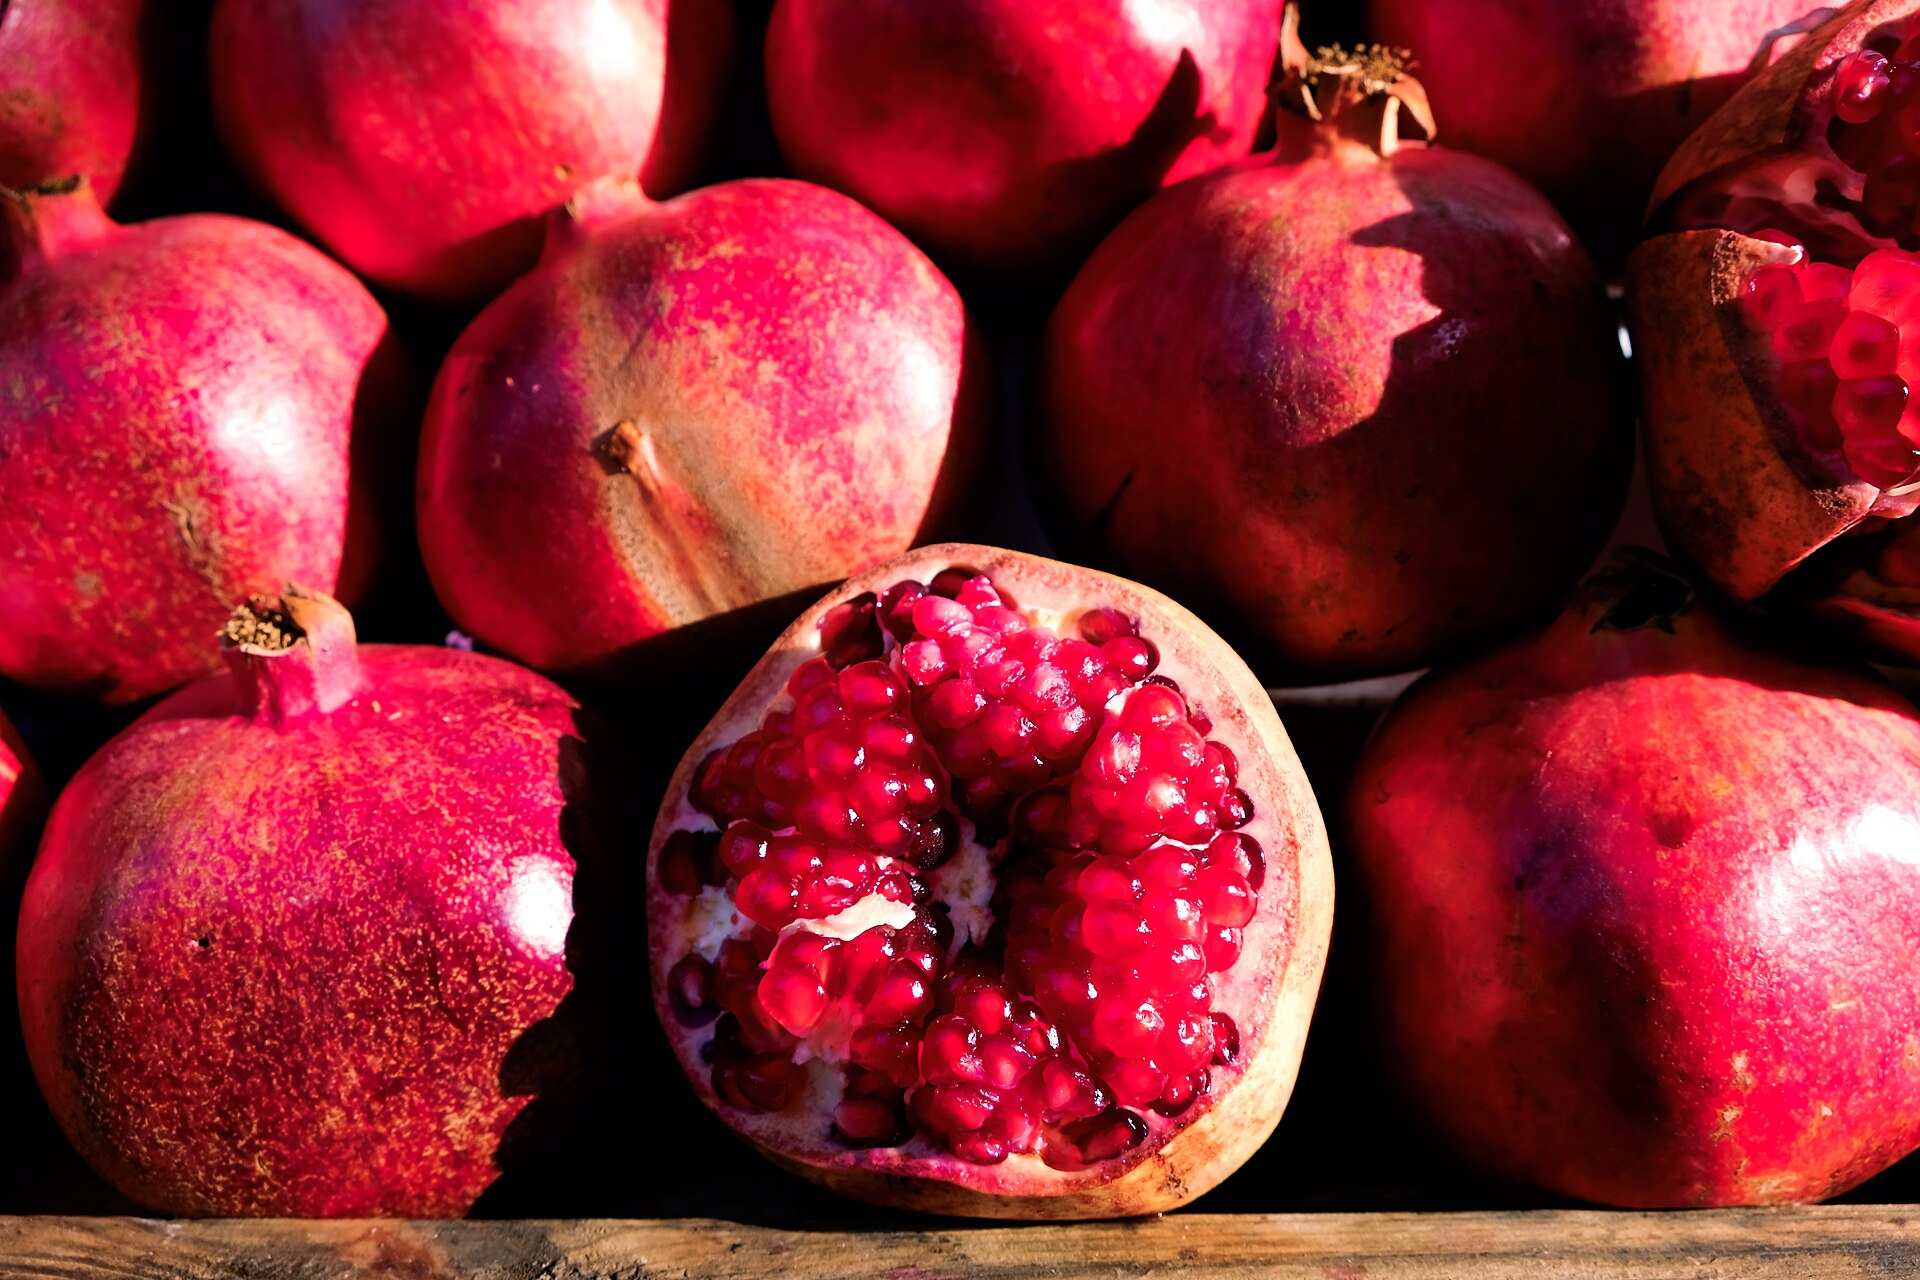
\includegraphics[width=0.94\linewidth]{pomegranate_market.jpg}
    \end{center}
  \end{columns}
\end{frame}

\begin{frame}{Outline}
  \tableofcontents
\end{frame}

% ================================================================
\section{One photo, four tasks}

\begin{frame}[plain]
  \vfill
  \begin{center}
    {\Large\color{popblue}\textbf{One photo, four tasks}}\\[0.9em]
    \begin{minipage}{0.82\textwidth}\centering\small
      What changes is the \emph{output}, not the backbone.
    \end{minipage}
  \end{center}
  \vfill
\end{frame}

\begin{frame}{The task zoo}
  \begin{center}
    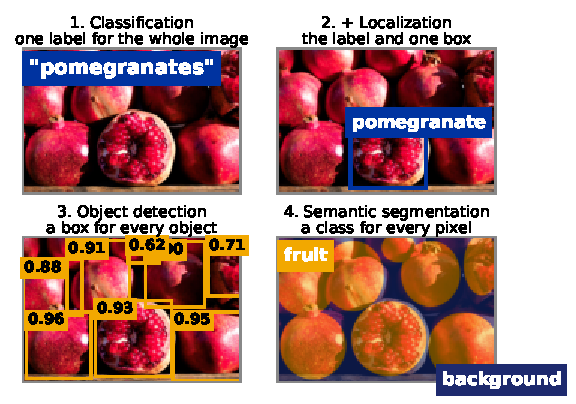
\includegraphics[height=2.25in]{task_zoo.pdf}
  \end{center}
  \vskip 2pt
  \fcolorbox{armblue}{armblue!8}{\parbox{0.97\linewidth}{\small
      Same photo, same conv backbone - four \textbf{output structures}: a label, a
      label $+$ a box, a box \emph{per object}, a class \emph{per pixel}. The output
      structure \emph{defines} the task. (Overlays drawn for illustration - no model
      ran on this photo.)}}
\end{frame}

% ================================================================
\section{Object detection}

\begin{frame}[plain]
  \vfill
  \begin{center}
    {\Large\color{popblue}\textbf{Object detection}}\\[0.9em]
    \begin{minipage}{0.82\textwidth}\centering\small
      What \emph{and} where - a class and a box for every object in the frame.
    \end{minipage}
  \end{center}
  \vfill
\end{frame}

\begin{frame}{From "what" to "what and where"}
  \begin{columns}[T]
    \column{0.44\textwidth}
    For \emph{one} object, no new machinery is needed - just a \textbf{longer label
    vector}:
    \[
      \yv =
      \begin{bmatrix}
        b_x\\ b_y\\ b_h\\ b_w\\ c_o\\ c_{\text{pom}}\\ c_{\text{apple}}\\ c_{\text{quince}}
      \end{bmatrix}
      \begin{matrix}
        \text{\footnotesize box center }x\\
        \text{\footnotesize box center }y\\
        \text{\footnotesize box height}\\
        \text{\footnotesize box width}\\
        \text{\footnotesize object present? (binary)}\\
        \text{\footnotesize class, one-hot}\\
        \text{\footnotesize class, one-hot}\\
        \text{\footnotesize class, one-hot}
      \end{matrix}
    \]
    \column{0.56\textwidth}
    Classification \textbf{and} box regression, one network: the box coordinates are
    just four regression outputs ([01]'s squared loss next to [11]'s log-loss).
    \vskip 6pt
    Box centre and size are \textbf{fractions of the photo} (0 to 1), so the same numbers
    work for any image size.
    \vskip 6pt
    \fcolorbox{armblue}{armblue!8}{\parbox{0.95\linewidth}{\small
      One entry looks odd: $c_o$, "is there an object at all?" Why would a fruit grader need
      a "no fruit" answer? Next slide.}}
  \end{columns}
\end{frame}

% 2026-10-14 addition (instructor: "explain why we need the cases where no object is present at
% all" and "clarify what you mean by confidence"). Confidence = the predicted c_o; the many-slots
% fix for "any number of objects" (moved here from the label-vector frame's old reveal).
\begin{frame}{"Nothing here" has to be an answer}
  \begin{columns}[T]
    \column{0.50\textwidth}
    \small
    \textbf{Predict:} the belt runs empty for a second - no fruit in the frame. What does the
    network output?
    \vskip 4pt
    \onslide<2->{%
    Without $c_o$ it \emph{cannot} say "none": every output is a box and a class, so it
    \textbf{invents a fruit} somewhere.
    \vskip 4pt
    With $c_o$, empty photos go into training too, labeled $c_o = 0$:
    \vskip 2pt
    {\footnotesize
    \begin{tabular}{r l}
      pomegranate: & $\yv = (.4, .6, .3, .2, \mathbf{1}, 1, 0, 0)$\\
      empty belt: & $\yv = (\,?,\ \,?,\ \,?,\ \,?,\ \mathbf{0}, ?, ?, ?)$
    \end{tabular}}
    \vskip 2pt
    The "?" entries are \textbf{don't care}: there is no box to learn, so the loss checks
    only $c_o$.}
    \column{0.48\textwidth}
    \onslide<2->{%
    \fcolorbox{armblue}{armblue!8}{\parbox{0.95\linewidth}{\small
      \textbf{Confidence} $=$ the network's \emph{predicted} $c_o$: a number from 0 to 1,
      "how sure am I that an object is here?" - [11]'s predicted probability, for the yes/no
      question "object or not". Every box a detector outputs carries one.}}}
    \vskip 6pt
    \onslide<3->{%
    \fcolorbox{armred}{armred!8}{\parbox{0.95\linewidth}{\small
      \textbf{The real reason:} a photo can hold \textbf{any number} of fruit, but a network
      has a \textbf{fixed output size}. The fix: give it many output \emph{slots}, each with
      its own $c_o$. Slots with a fruit fill in a box; every other slot answers
      $c_o = 0$, "nothing here". That is a detector.}}}
  \end{columns}
\end{frame}

% 2026-10-02 addition (instructor: "how come detectors output many boxes? one would expect just
% one answer"). detector_candidates.py runs a real detector (torchvision SSDlite320, COCO) on the
% belt photo; every count here is in results/detector_candidates.json. YOLOv8 at 640 px:
% 80^2 + 40^2 + 20^2 = 8,400 predictions.
\begin{frame}{Why a detector answers with so many boxes}
  \par\vskip 2pt{\centering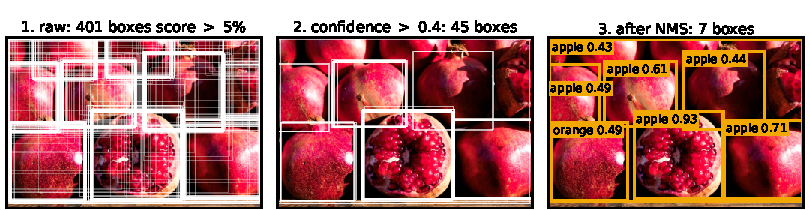
\includegraphics{detector_candidates.pdf}\par}
  \vskip 4pt
  \begin{columns}[T]
    \column{0.55\textwidth}
    \footnotesize
    \begin{enumerate}\setlength\itemsep{0pt}
      \item The slots from the last slide: a fixed set of \textbf{candidate} boxes, each with
        a \textbf{confidence}. This model: 3{,}234 for every photo. YOLO v1: 98. YOLOv8:
        8{,}400.
      \item Most candidates look at background: low confidence, cut by a
        \textbf{threshold}.
      \item A fruit covers many positions, and each nearby candidate finds it:
        \textbf{duplicates}. NMS keeps the best one per object (two slides on).
    \end{enumerate}
    \column{0.43\textwidth}
    \footnotesize
    A real detector (SSDlite, trained on COCO) on our photo. COCO has no pomegranate class,
    so it says "apple" - and boxes the whole crate as one more apple.
    \vskip 3pt
    \fcolorbox{armblue}{armblue!8}{\parbox{0.95\linewidth}{\footnotesize
      The many boxes are the \textbf{raw} output, not the answer. The answer is what survives
      the threshold and NMS.}}
  \end{columns}
\end{frame}

% 2026-10-14 additions (instructor: "how are those boxes even obtained? does one run the same
% model for a ton of boxes? does that mean a fixed box size? spend more frames"). All numbers from
% py_src/candidate_boxes.py -> results/candidate_boxes.json: 120 crops (3 sizes, stride half a
% window) through ImageNet ResNet-18, 12.2 s on this laptop's CPU; SSDlite320 grids 20,10,5,3,2,1
% x 6 anchors = 3,234; top candidate = 5x5 grid, cell (3, 2), anchor 160x160 on the 320x320 input,
% shift (+3.4, -3.2) px, stretch x0.70 / x1.02, "apple" 0.93 (= the 0.93 of detector_candidates).
% R-CNN: Girshick et al., arXiv 1311.2524 v5: "around 2000 region proposals", "13s/image on a GPU
% or 53s/image on a CPU".
\begin{frame}{Where candidates come from - idea 1: crop and classify}
  \begin{columns}[T]
    \column{0.50\textwidth}
    {\centering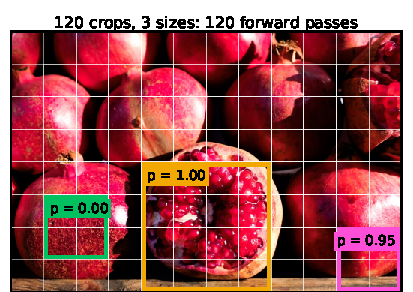
\includegraphics[width=\linewidth]{sliding_windows.pdf}\par}
    \vskip 1pt
    {\scriptsize $p$ $=$ ImageNet ResNet-18's probability of "pomegranate" for that crop.
    White grid: the smallest windows, overlapping by half.}
    \column{0.48\textwidth}
    \small
    The obvious detector: slide a \textbf{window} over the photo at several sizes, crop, and
    run a \textbf{classifier} on every crop. A high score means "fruit here" - the window
    \emph{is} the box.
    \vskip 3pt
    Measured on our photo: \textbf{120 crops, 120 forward passes}, 12 s on a laptop CPU. Real
    detectors need more sizes, shapes and positions: thousands of crops.
    \vskip 3pt
    \textbf{R-CNN} (2014) did exactly this, on $\sim$\textbf{2,000} smart crops per photo:
    \textbf{13 s per image} on a GPU.
    \vskip 3pt
    \fcolorbox{armred}{armred!8}{\parbox{0.95\linewidth}{\small
      So yes: the first detectors ran one model on a ton of boxes. The waste: overlapping
      crops recompute the same pixels again and again.}}
  \end{columns}
\end{frame}

\begin{frame}{Idea 2: one pass, a small head at every cell}
  \begin{columns}[T]
    \column{0.50\textwidth}
    {\centering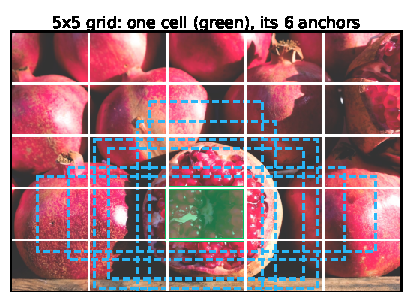
\includegraphics[width=\linewidth]{ssd_grid_anchors.pdf}\par}
    \vskip 1pt
    {\scriptsize The real model from the many-boxes slide (SSDlite). Dashed: preset box
    shapes, \textbf{anchors}, centred on the green cell.}
    \column{0.48\textwidth}
    \small
    Run the backbone \textbf{once}. Its last maps form a grid - like [50]'s $7\times7\times512$
    - and each cell's vector describes the photo \emph{around} that cell.
    \vskip 3pt
    Put a small conv layer, the \textbf{head}, on the grid. A conv slides by construction
    ([48]), so the head runs at \textbf{every cell} in the same pass, reusing the backbone's
    work.
    \vskip 3pt
    Per cell, for each of its 6 anchors: \textbf{4 box numbers} $+$ \textbf{91 class
    scores} (one class is "background": SSD's "nothing here").
    \vskip 3pt
    \fcolorbox{armblue}{armblue!8}{\parbox{0.95\linewidth}{\small
      6 grids, fine to coarse ($20\times20$ for small fruit \dots\ $1\times1$ for the whole
      photo): $(400 + 100 + 25 + 9 + 4 + 1) \times 6 = \mathbf{3{,}234}$ candidates.}}
  \end{columns}
\end{frame}

\begin{frame}{Box sizes are not fixed: anchors + offsets}
  \begin{columns}[T]
    \column{0.48\textwidth}
    {\centering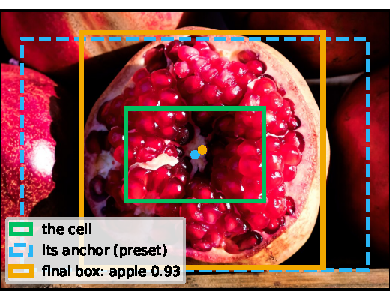
\includegraphics[width=\linewidth]{ssd_anchor_decode.pdf}\par}
    \vskip 1pt
    {\scriptsize The top candidate on our photo, zoomed. COCO has no pomegranate class.}
    \column{0.50\textwidth}
    \small
    An anchor is only a \textbf{starting guess}. The head \textbf{regresses} ([01]) how to fix
    it: shift the centre, stretch the width and height,
    \[
      w = w_{\text{anchor}} \cdot e^{t_w}, \qquad h = h_{\text{anchor}} \cdot e^{t_h}
    \]
    ($e^{t}$: any stretch factor, never negative).
    \vskip 2pt
    This fruit, measured: anchor $160\times160$ on the model's $320\times320$ input; the head
    said \textbf{move 3 px, stretch $\times 0.70$ and $\times 1.02$} $\to$ a $111\times163$
    box, "apple" $0.93$.
    \vskip 4pt
    \fcolorbox{paramgreen}{paramgreen!8}{\parbox{0.95\linewidth}{\small
      No fixed box size: the anchor sets roughly where and how big, the network fixes the
      rest. And no box has to fit inside its cell - this one is $1.7 \times 2.5$ cells.}}
  \end{columns}
\end{frame}

\begin{frame}{IoU: the overlap score}
  \begin{columns}[T]
    \column{0.44\textwidth}
    Detectors output many boxes, so we constantly ask: \textbf{how much do two boxes
    agree?}
    \[
      \text{IoU}(A, B) = \frac{\text{area}(A \cap B)}{\text{area}(A \cup B)}
    \]
    $1$ = identical boxes, $0$ = no overlap; in practice $\text{IoU} \ge 0.5$ usually
    counts as "the same object".
    \vskip 6pt
    \fcolorbox{armblue}{armblue!8}{\parbox{0.95\linewidth}{\small
      Worked example: $A = (0,0)$-$(4,4)$, $B = (2,0)$-$(6,4)$. Intersection $= 8$,
      union $= 16 + 16 - 8 = 24$, so $\text{IoU} = 8/24 = \mathbf{1/3}$.}}
    \column{0.56\textwidth}
    \begin{center}
      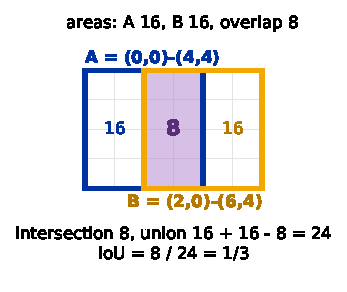
\includegraphics[width=0.9\linewidth]{iou_only.pdf}
    \end{center}
  \end{columns}
\end{frame}

% 2026-10-01: two columns so the animation gets 3 in instead of 2.1 in (its badges rendered at
% 2.6 pt); nms_anim.py / iou_nms.py redrawn at that size.
\begin{frame}{NMS: from a flood of boxes to a clean answer}
  \begin{columns}[T]
    \column{0.42\textwidth}
    \small
    A detector proposes \textbf{many overlapping candidates} per object.
    \textbf{Non-max suppression} cleans up. \textbf{(Click to advance.)}
    \vskip 6pt
    \fcolorbox{armblue}{armblue!8}{\parbox{0.95\linewidth}{\small
      \textbf{Keep} the highest-scoring box, \textbf{drop} every neighbor whose IoU with it
      exceeds a threshold (here $0.45$), repeat. Too high: duplicates survive. Too low:
      touching fruit lose a box.}}
    \vskip 6pt
    {\footnotesize \textbf{2026:} the newest detectors are \emph{trained} to emit one box per
    object and skip NMS - DETR, the detection transformer (Carion et al., 2020), and
    Ultralytics' YOLO26 (Jan 2026). The duplicates did not go away; the model learned to
    suppress them itself.}
    \column{0.56\textwidth}
    \begin{center}
      \only<1>{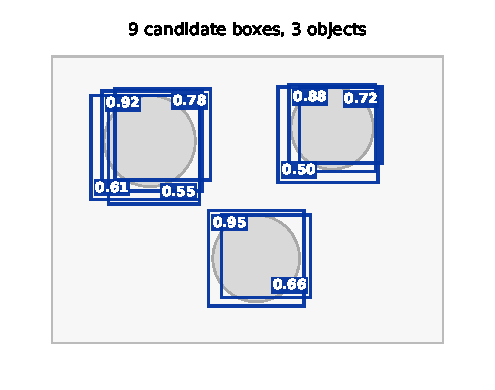
\includegraphics[width=\linewidth]{nms_anim_0.pdf}}%
      \only<2>{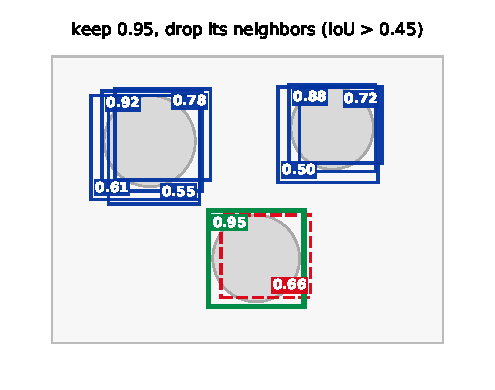
\includegraphics[width=\linewidth]{nms_anim_1.pdf}}%
      \only<3>{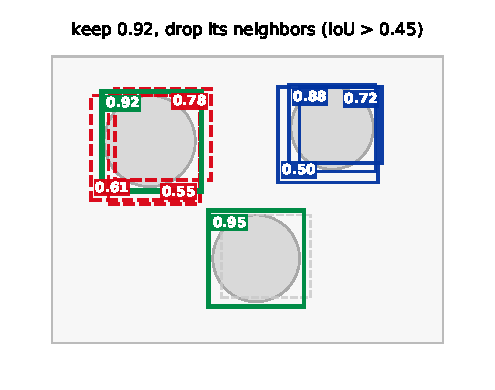
\includegraphics[width=\linewidth]{nms_anim_2.pdf}}%
      \only<4>{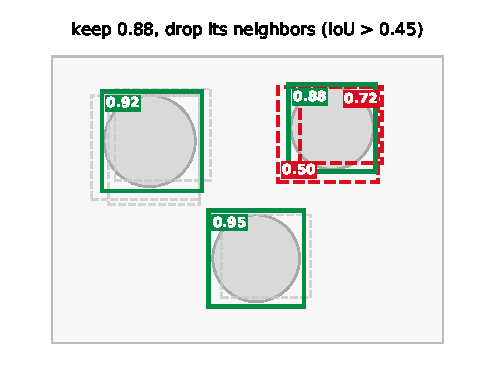
\includegraphics[width=\linewidth]{nms_anim_3.pdf}}%
      \only<5>{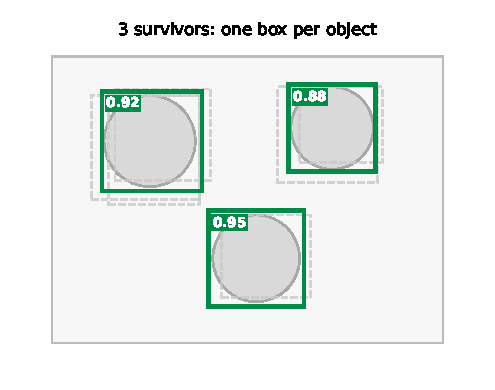
\includegraphics[width=\linewidth]{nms_anim_4.pdf}}%
    \end{center}
  \end{columns}
\end{frame}

\begin{frame}{Scoring a detector: mAP in one line}
  \begin{itemize}
    \item A predicted box is \textbf{correct} if the class matches and its IoU with a
      true box passes a threshold (say $0.5$).
    \item That makes every prediction a TP or FP - so \textbf{precision} and
      \textbf{recall} are exactly [12]'s, computed over boxes.
    \item \textbf{AP} $=$ area under the precision-recall curve, per class;
      \textbf{mAP} $=$ the mean over classes. Benchmarks also sweep the IoU threshold
      ($0.5$ to $0.95$) and average once more.
  \end{itemize}
  \vskip 8pt
  \fcolorbox{armblue}{armblue!8}{\parbox{0.97\linewidth}{\small
      No new metric theory: mAP is the \textbf{[12] machinery wrapped around boxes},
      swept over IoU thresholds.}}
\end{frame}

% 2026-09-22 addition (student review: "mAP is vocabulary, not a skill"). Numbers computed
% in the session scratchpad: P = 1, .5, .667, .5; R = .5, .5, 1, 1; AP = .5*1 + .5*.667 = .833;
% reversed ranking (FP, FP, TP, TP) gives AP = .5*(1/3) + .5*(1/2) = .417 (sklearn
% average_precision_score agrees; the .5 stated here until 2026-09-30 was the INTERPOLATED AP).
\begin{frame}{mAP by hand}
  \small
  One class, \textbf{2} true pomegranates in the photo. The detector returns 4 boxes;
  sort them by score and mark each \textbf{TP} (IoU $\ge 0.5$ with a not-yet-matched true
  box) or \textbf{FP}:
  \vskip 4pt
  \begin{columns}[T]
    \column{0.50\textwidth}
    \begin{center}\footnotesize
      \begin{tabular}{c c c c c}
        \textbf{rank} & \textbf{score} & & \textbf{precision} & \textbf{recall}\\
        \hline
        1 & 0.9 & TP & $1/1 = 1.00$ & $1/2 = 0.50$\\
        2 & 0.8 & FP & $1/2 = 0.50$ & $0.50$\\
        3 & 0.7 & TP & $2/3 = 0.67$ & $2/2 = 1.00$\\
        4 & 0.6 & FP & $2/4 = 0.50$ & $1.00$\\
      \end{tabular}
    \end{center}
    \column{0.46\textwidth}
    \textbf{AP} $=$ area under the precision-recall steps - each TP adds its recall gain
    times its precision:
    \[
      \text{AP} = 0.5 \times 1.00 + 0.5 \times 0.67 = \mathbf{0.83}
    \]
    \textbf{mAP} $=$ the mean over classes: if apples score $0.60$,
    $\text{mAP} = (0.83 + 0.60)/2 \approx 0.72$.
  \end{columns}
  \vskip 6pt
  \fcolorbox{armblue}{armblue!8}{\parbox{0.97\linewidth}{\small
    \textbf{Ranking matters}: the same four boxes with the two false alarms scored highest
    give AP~$= 0.5 \times \tfrac13 + 0.5 \times \tfrac12 \approx 0.42$ - half the score. mAP rewards finding every object \emph{and} being most confident about
    the right ones. (COCO then also averages over IoU thresholds $0.50$ to $0.95$.)}}
\end{frame}

% ================================================================
% 2026-10-14 (instructor: "transitions are too abrupt, e.g. before two families of detectors"):
% the detector internals became their own section with a transition slide.
\section{Building a detector}

\begin{frame}[plain]
  \vfill
  \begin{center}
    {\Large\color{popblue}\textbf{Two ways to build a detector}}\\[0.9em]
    \begin{minipage}{0.82\textwidth}\centering\small
      You know what a detector outputs and how it is scored. Crop-and-classify and
      one-pass-over-a-grid were not just ideas: they are the two families of real detectors.
      One of them became the industry default.
    \end{minipage}
  \end{center}
  \vfill
\end{frame}

\begin{frame}{Two families of detectors}
  \begin{columns}[T]
    \column{0.5\textwidth}
    \textbf{Two-stage} $=$ idea 1, made fast: first \emph{propose} candidate regions, then
    classify and refine each.
    \begin{itemize}
      \item R-CNN (2014) $\to$ Fast $\to$ \textbf{Faster R-CNN} (2015)
      \item accurate, but two passes of work
    \end{itemize}
    \column{0.5\textwidth}
    \textbf{One-stage} $=$ idea 2: predict all boxes and classes in \emph{one} forward pass.
    \begin{itemize}
      \item \textbf{YOLO} ("You Only Look Once", 2016), SSD (Single Shot MultiBox
        Detector, 2016)
      \item real-time - video-rate detection
    \end{itemize}
  \end{columns}
  \vskip 8pt
  \fcolorbox{armblue}{armblue!8}{\parbox{0.97\linewidth}{\small
      Two-stage bought \textbf{accuracy}, one-stage bought \textbf{speed} - and a decade
      of iteration has mostly closed the gap.}}
  \vskip 6pt
  In practice, YOLO became the industry default: you \texttt{pip install} a pretrained
  one and fine-tune it on \emph{your} boxes ([50]'s recipe). That \textbf{is} the sorting
  line's counting camera.
  \vskip 4pt
  {\scriptsize\color{gray} Girshick et al. 2014; Ren et al. 2015; Redmon et al. 2016;
  Liu et al. 2016.}
\end{frame}

\begin{frame}{How one-stage works: the YOLO grid}
  \begin{columns}[T]
    \column{0.42\textwidth}
    \begin{itemize}
      \item Divide the image into an $S \times S$ grid ($7 \times 7$ in the paper).
      \item \textbf{Each cell} predicts $2$ candidate boxes - $(x, y, w, h,
        \text{confidence})$ - plus class probabilities. Confidence: the predicted $c_o$, trained
        towards how well the box fits (its IoU with the truth).
      \item All $98$ boxes come out of \textbf{one forward pass}, as one $7 \times 7
        \times 30$ tensor. That is why it runs in real time.
    \end{itemize}
    \vskip 4pt
    \fcolorbox{armblue}{armblue!8}{\parbox{0.95\linewidth}{\small
      A flood of overlapping candidates by \emph{design} - exactly why \textbf{NMS}
      exists.}}
    \column{0.58\textwidth}
    \begin{center}
      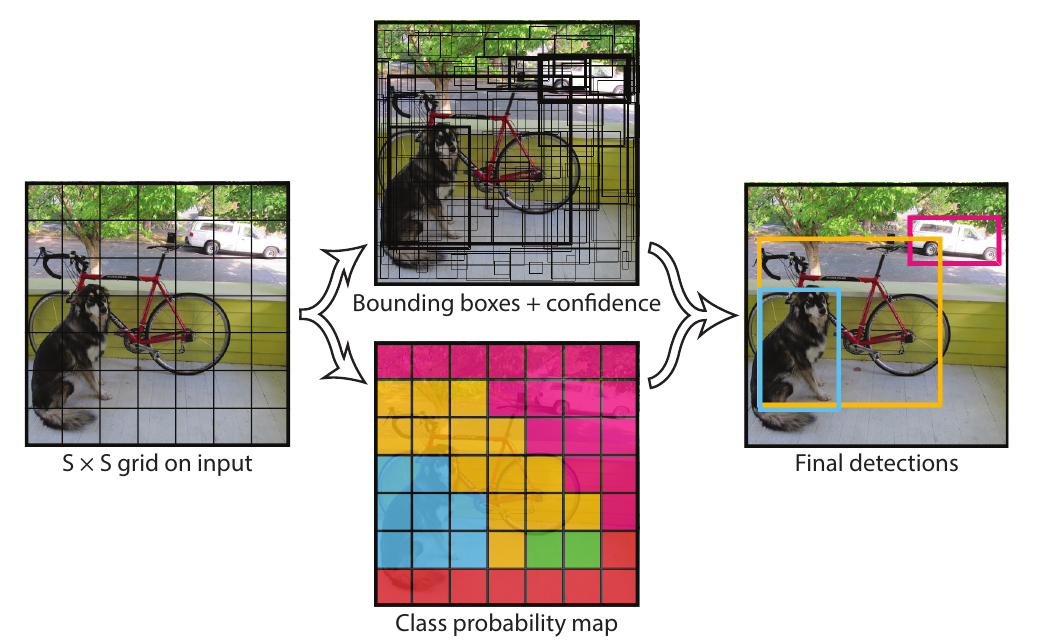
\includegraphics[width=0.92\linewidth]{yolo_grid.png}\\[2pt]
      {\scriptsize The paper's own diagram (Redmon et al., "You Only Look Once",
      2016).}
    \end{center}
  \end{columns}
\end{frame}

% 2026-09-22 addition (student review: "how does one tensor become a pixel box?"). Facts from
% Redmon et al. 2016, arXiv 1506.02640: 448x448 input; (x, y) = box centre relative to the
% grid cell; (w, h) relative to the whole image; class-specific score = Pr(class|object) *
% confidence; the "responsible" predictor = highest IoU with the ground truth.
% 2026-10-14 (instructor: "add the YOLO founder's CV, it's hilarious"). Resume = pjreddie.com/static/
% resume.pdf rendered at 200 dpi -> fig/borrowed/redmon_resume.png. YOLOv3 quote and the Newton
% citation: arXiv 1804.02767 (intro; reference [12] is Newton's Principia). 2020 quote: Redmon on
% Twitter, Feb 2020, reported by The Batch (deeplearning.ai, "Code No Evil"). YOLOv4: Bochkovskiy
% et al. 2020; YOLOv5 onward: Ultralytics.
\begin{frame}{Meet YOLO's author}
  \begin{columns}[T]
    \column{0.6\textwidth}
    \small
    \textbf{Joseph Redmon}, PhD student at the University of Washington: YOLO (2016),
    YOLO9000 (2017) and YOLOv3 (2018), all in his own C framework, Darknet.
    \vskip 4pt
    His CV (right) is a My Little Pony fan page: "This little pony went to Middlebury
    College..."
    \vskip 4pt
    The YOLOv3 paper opens: \emph{"Sometimes you just kinda phone it in for a year, you know?
    I didn't do a whole lot of research this year. Spent a lot of time on Twitter."} It cites
    Newton's \emph{Principia} for the word "momentum".
    \vskip 6pt
    \fcolorbox{armorange}{armorange!12}{\parbox{0.95\linewidth}{\small
      The serious end: in 2020 he quit computer vision - "the military applications and
      privacy concerns eventually became impossible to ignore." YOLO v4 onward is other
      people's work; today mostly Ultralytics'.}}
    \column{0.38\textwidth}
    \begin{center}
      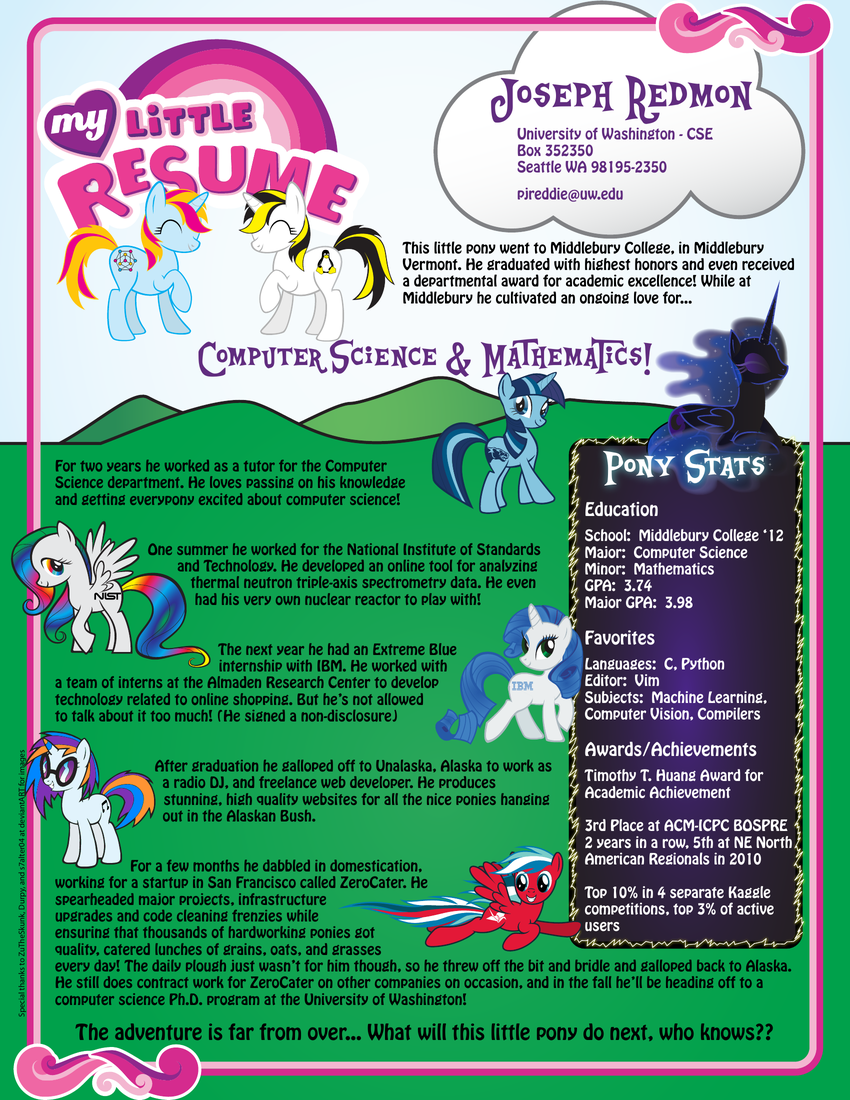
\includegraphics[height=0.72\textheight]{redmon_resume.png}\\[1pt]
      {\scriptsize\color{gray} pjreddie.com/static/resume.pdf}
    \end{center}
  \end{columns}
\end{frame}

% 2026-10-14 (instructor: "how can a small cell holding part of the object, like a dog's belly,
% predict anything, and how is the final box bigger than the cell?"). yolo_cell_figs.py. Redmon
% et al. 2016, Sec. 2: the network "uses features from the entire image to predict each bounding
% box"; 24 conv layers followed by 2 fully connected layers.
\begin{frame}{A cell is an address, not a window}
  {\centering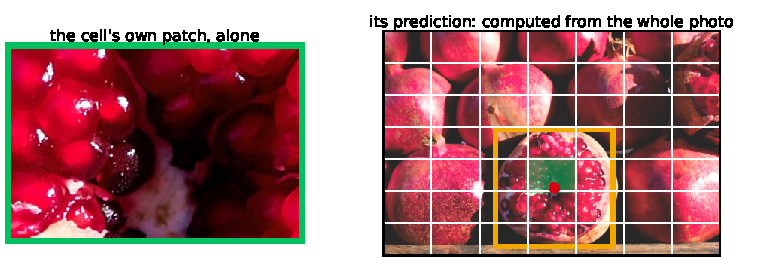
\includegraphics[width=0.78\linewidth]{yolo_address.pdf}\par}
  \vskip 2pt
  \begin{columns}[T]
    \column{0.52\textwidth}
    \small
    Alone, the cell's patch (left) is a slab of seeds - like the dog's belly in the paper's
    photo. Nobody could tell where the fruit ends.
    \vskip 3pt
    But YOLO v1 ends in two \textbf{fully connected} layers: every number of every cell is
    computed from \textbf{every pixel}.
    \column{0.46\textwidth}
    \fcolorbox{armblue}{armblue!8}{\parbox{0.95\linewidth}{\small
      The grid decides \textbf{who reports} an object: the cell holding its centre. The whole
      network decides \textbf{what} gets reported - so the box can be far bigger than the
      cell.}}
  \end{columns}
\end{frame}

\begin{frame}{Decoding one YOLO cell, by hand}
  \begin{columns}[T]
    \column{0.40\textwidth}
    {\centering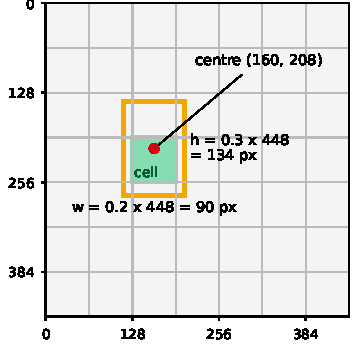
\includegraphics[width=\linewidth]{yolo_decode.pdf}\par}
    \column{0.58\textwidth}
    \small
    YOLO squashes every photo to $448\times448$: 49 cells of $64$ px. One box of the green
    cell (row 3, column 2) outputs:
    \vskip 3pt
    \begin{tabular}{l l}
      $x = 0.5,\ y = 0.25$ & centre, as fractions of the \textbf{cell}\\
      $w = 0.2,\ h = 0.3$ & size, as fractions of the \textbf{image}\\
      confidence $0.8$, & $P(\text{pomegranate} \mid \text{object}) = 0.9$
    \end{tabular}
    \vskip 5pt
    \begin{itemize}\setlength\itemsep{2pt}
      \item centre: $\big((2 + 0.5)\cdot 64,\ (3 + 0.25)\cdot 64\big) = (160, 208)$
      \item size: $90 \times 134$ px - wider and taller than the 64 px cell
      \item score: $0.8 \times 0.9 = \mathbf{0.72}$, the number NMS sorts by
    \end{itemize}
  \end{columns}
\end{frame}

% 2026-10-13 addition (the deck stated the "any number of objects vs fixed output size" mismatch
% and solved it only for inference). Facts from Redmon et al. 2016 (arXiv 1506.02640, Sec. 2 and
% 2.2): "If the center of an object falls into a grid cell, that grid cell is responsible for
% detecting that object"; "in every image many grid cells do not contain any object. This pushes
% the 'confidence' scores of those cells towards zero, often overpowering the gradient from cells
% that do contain objects. This can lead to model instability, causing training to diverge early
% on"; lambda_coord = 5, lambda_noobj = .5; confidence target = IOU(pred, truth). Counts from
% py_src/yolo_targets.py (asserted): 8 hand-placed fruit -> 8 distinct responsible cells; 98
% predictors; 90 trained towards confidence 0. Focal loss: Lin, Goyal, Girshick, He, Dollar,
% ICCV 2017 (arXiv 1708.02002).
\begin{frame}{Training the grid: who learns what}
  \begin{columns}[T]
    \column{0.50\textwidth}
    {\centering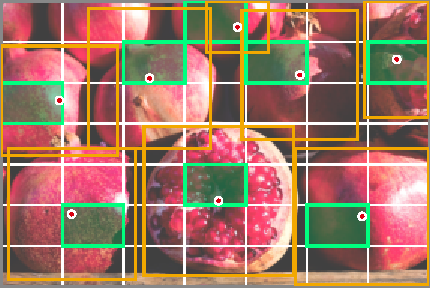
\includegraphics[width=0.88\linewidth]{yolo_targets.pdf}\par}
    \vskip 1pt
    {\scriptsize Orange: true boxes. Green: the cell holding a fruit's centre (red dot).}
    \vskip 4pt
    \fcolorbox{armblue}{armblue!8}{\parbox{0.95\linewidth}{\small
      A fixed-size output learning from \textbf{any number} of objects: each true box goes
      into its responsible slot; every other slot learns "nothing here".}}
    \column{0.48\textwidth}
    \small
    YOLO's rule: the cell holding a fruit's \textbf{centre} is responsible for it - and of
    its two predictors, the one that already overlaps it best.
    \vskip 3pt
    On this photo: 8 fruit $\to$ \textbf{8} responsible predictors of 98.
    \begin{itemize}\setlength\itemsep{1pt}
      \item those 8: box loss, class loss, confidence $\to$ their IoU with the truth;
      \item the other \textbf{90}: confidence $\to 0$, box "don't care".
    \end{itemize}
    \vskip 2pt
    \fcolorbox{armred}{armred!8}{\parbox{0.95\linewidth}{\small
      \textbf{90 "nothing" vs 8 "fruit"}: [12]'s class imbalance. The empty cells' gradients
      made training diverge, so YOLO weights them by $\lambda_{\text{noobj}} = 0.5$ (box
      errors by $\lambda_{\text{coord}} = 5$). Later: the \textbf{focal loss} (Lin et al.,
      2017) shrinks the loss of easy background.}}
  \end{columns}
\end{frame}

% 2026-10-14 (instructor: "clarify what loss is used in object detection - there is both regression
% and classification"). YOLO v1 (arXiv 1506.02640, Sec. 2.2): "We use sum-squared error because it
% is easy to optimize"; "we predict the square root of the bounding box width and height";
% lambda_coord 5, lambda_noobj .5. Modern YOLO = Ultralytics v8DetectionLoss (ultralytics/utils/
% loss.py, read 2026-10-14): BCEWithLogitsLoss for classes, bbox_iou(..., CIoU=True) for boxes,
% no separate objectness term.
\begin{frame}{The detection loss: regression and classification, added}
  \small
  \textbf{Predict:} a detector outputs box numbers (regression) \emph{and} class scores
  (classification). Which loss does it train with?
  \vskip 4pt
  \onslide<2->{%
  \textbf{Both, added.} Each output gets the loss that fits its type; one backward pass trains
  them all:
  \vskip 4pt
  \begin{center}\footnotesize
    \begin{tabular}{l l l l}
      \textbf{part} & \textbf{which slots} & \textbf{YOLO v1 (2016)} & \textbf{modern YOLO}\\
      \hline
      box $x, y, w, h$ & responsible only & squared error ([01]), weight 5 & IoU-based loss\\
      confidence & all; empty ones $\times 0.5$ & squared error to IoU or 0 & inside the class scores\\
      class & cells with an object & squared error & log-loss ([11])\\
    \end{tabular}
  \end{center}
  \vskip 2pt
  \[
    L = \lambda_{\text{coord}}\, L_{\text{box}} + L_{\text{conf}} + L_{\text{class}}
  \]}
  \vskip -4pt
  \onslide<3->{%
  \begin{columns}[T]
    \column{0.5\textwidth}
    \fcolorbox{armorange}{armorange!12}{\parbox{0.95\linewidth}{\footnotesize
      YOLO v1 used squared error even for classes, "because it is easy to optimize". On
      $\sqrt{w}, \sqrt{h}$: a 10 px miss matters on a small fruit, not on a big crate.}}
    \column{0.48\textwidth}
    \fcolorbox{paramgreen}{paramgreen!8}{\parbox{0.95\linewidth}{\footnotesize
      The $\lambda$ weights set how much each part counts - the knob from the last slide.}}
  \end{columns}}
\end{frame}

% 2026-10-13 addition: cashes [50]'s "boxes cost money" thread. Ultralytics "Tips for Best
% Training Results" (docs.ultralytics.com/yolov5/tutorials/tips_for_best_training_results/,
% checked 2026-10-13): >= 1500 images per class, >= 10000 labeled instances per class, every
% instance of every class in every image must be labeled. YOLO v1 pretrained its
% conv layers on ImageNet (paper Sec. 2.2). YOLO-World: Cheng et al., arXiv 2401.17270 (CVPR
% 2024), real-time open-vocabulary detection. SAM 3 "Segment Anything with Concepts": Meta,
% released 2025-11-19, text or exemplar prompt -> masks and IDs for every matching instance.
\begin{frame}{Your own detector: label boxes, or prompt for them}
  \small
  \textbf{Route 1 - fine-tune a pretrained YOLO on your boxes} ([50]'s recipe; YOLO v1
  itself started from ImageNet-pretrained convs). Ultralytics' advice for good results:
  $\ge 1{,}500$ images and $\ge 10{,}000$ labeled boxes \emph{per class}.
  \vskip 4pt
  \fcolorbox{armred}{armred!8}{\parbox{0.97\linewidth}{\small
    \textbf{Label every fruit in every photo.} An unlabeled fruit is not "missing data": its
    cell is trained to say \textbf{"nothing here"}. Half-labeled photos teach the detector to
    ignore fruit.}}
  \vskip 6pt
  \textbf{Route 2 - prompt instead of label.} \emph{Open-vocabulary} models take the classes as
  \textbf{text}: YOLO-World (Cheng et al., 2024) detects whatever names you type, no boxes
  needed; SAM 3 (Meta, Nov 2025) returns a mask for every instance of a typed concept.
  \vskip 6pt
  \fcolorbox{paramgreen}{paramgreen!8}{\parbox{0.97\linewidth}{\small
    \textbf{In practice, both:} prompt a big model to \emph{draft} the boxes, people correct
    them, then fine-tune a small, fast YOLO for the belt camera. [50]'s price of boxes, cut
    twice.}}
\end{frame}

% 2026-10-14 (instructor: "explain separable convs better, and why are you even mentioning them").
% Figure: py_src/separable_idea.py (weights asserted: 19,200 vs 75 + 768 = 843). SSDlite-MobileNetV3
% (the many-boxes slide's model): MobileNetV3 blocks are built on depthwise convs, and SSDlite
% replaces the SSD head's regular convs with depthwise separable ones (MobileNetV2 paper).
\begin{frame}{Making it fast: separable convolutions}
  \small
  \textbf{Why here?} The belt camera needs boxes for every frame - 30 a second, on a small
  computer, no data centre. The detector from the many-boxes slide, \textbf{SSDlite-MobileNetV3},
  is phone-sized because it is built from \emph{separable} convolutions.
  \vskip 2pt
  {\centering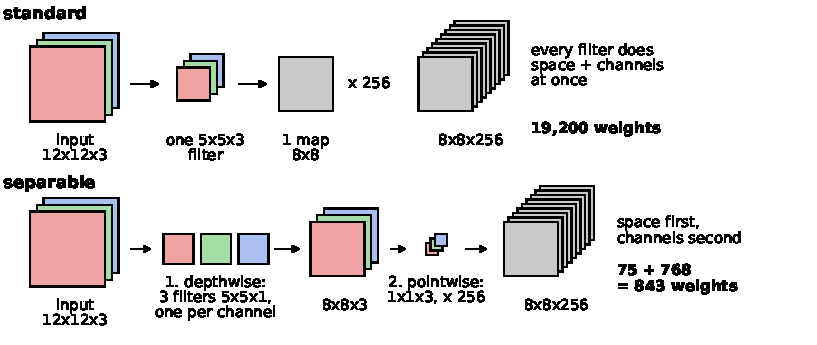
\includegraphics[width=0.8\linewidth]{separable_idea.pdf}\par}
  \vskip 2pt
  \fcolorbox{armblue}{armblue!8}{\parbox{0.97\linewidth}{\small
    First each channel is filtered \textbf{alone} (space), then $1\times1$ convs ([49])
    \textbf{mix} the channels. Less flexible than a standard filter, far cheaper: next slide.}}
\end{frame}

\begin{frame}{Separable convolutions: the count}
  \begin{columns}[T]
    \column{0.47\textwidth}
    Input $12 \times 12 \times 3$, $5\times5$ filters, $256$ output channels
    $\Rightarrow$ output $8 \times 8$. Count multiplications:
    \vskip 4pt
    {\small
    \textbf{Standard:}
    \[
      256 \cdot \underbrace{(5 \cdot 5 \cdot 3)}_{\text{per stop}} \cdot
      \underbrace{(8 \cdot 8)}_{\text{stops}} = \mathbf{1{,}228{,}800}
    \]
    \textbf{Depthwise} $+$ \textbf{pointwise}:
    \[
      \underbrace{3 \cdot 25 \cdot 64}_{4{,}800} +
      \underbrace{256 \cdot 3 \cdot 64}_{49{,}152} = \mathbf{53{,}952}
    \]}
    \column{0.53\textwidth}
    \begin{center}
      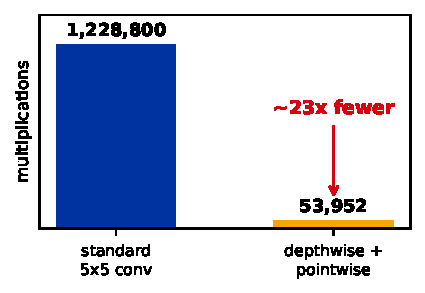
\includegraphics[width=0.94\linewidth]{separable_count.pdf}
    \end{center}
  \end{columns}
  \vskip 2pt
  \fcolorbox{paramgreen}{paramgreen!8}{\parbox{0.97\linewidth}{\small
      $\sim$\textbf{23}$\times$ fewer multiplications for the same output shape. This is
      why a pretrained detector runs \emph{on} the sorting line, not in a cloud.}}
  \vskip 2pt
  {\scriptsize\color{gray} Not the same as a \emph{spatially} separable kernel (Sobel $=$
  column $\times$ row, [48]): that one splits space; this one splits space from channels.}
\end{frame}

% ================================================================
\section{Segmentation}

\begin{frame}[plain]
  \vfill
  \begin{center}
    {\Large\color{popblue}\textbf{Segmentation}}\\[0.9em]
    \begin{minipage}{0.82\textwidth}\centering\small
      Every pixel gets an answer.
    \end{minipage}
  \end{center}
  \vfill
\end{frame}

\begin{frame}{Semantic vs instance}
  \begin{columns}[T]
    \column{0.42\textwidth}
    Segmentation $=$ \textbf{per-pixel classification}.
    \vskip 4pt
    \begin{itemize}
      \item \textbf{Semantic}: every pixel gets a class label - all our pomegranates
        merge into \emph{one} fruit mask (task-zoo panel 4).
      \item \textbf{Instance}: each fruit gets its \textbf{own} mask.
        \textbf{Mask R-CNN} $=$ Faster R-CNN $+$ a small mask head per region
        (He et al., 2017).
      \item \textbf{Panoptic}: both at once - every pixel labeled \emph{and} grouped
        into instances.
    \end{itemize}
    \column{0.58\textwidth}
    \begin{center}
      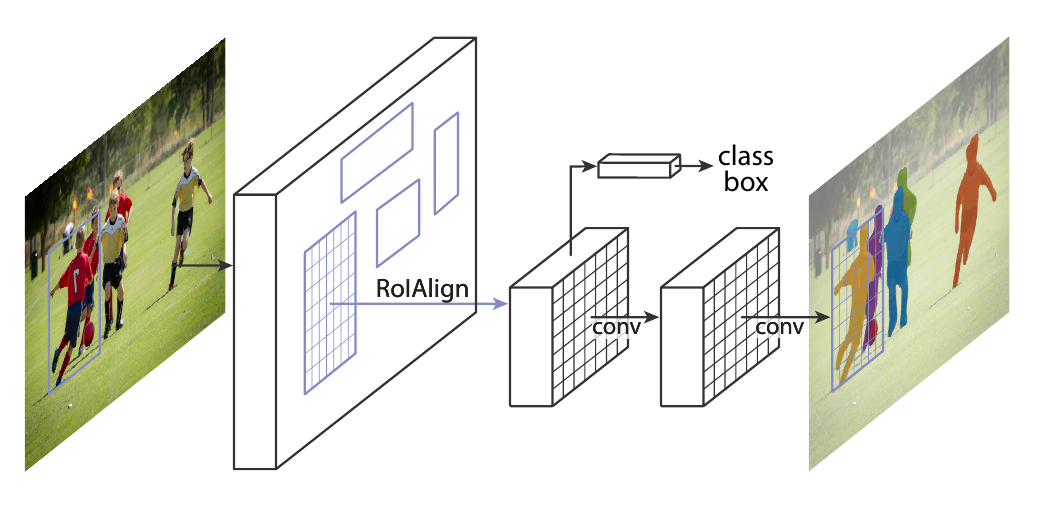
\includegraphics[width=0.93\linewidth]{maskrcnn_framework.png}\\[2pt]
      {\scriptsize Mask R-CNN: detection boxes plus a per-region mask branch
      (He et al., 2017).}
    \end{center}
    \vskip 3pt
    \fcolorbox{armblue}{armblue!8}{\parbox{0.95\linewidth}{\small
      From the [49] epilogue: \textbf{SAM 3} (Meta, 2025) made segmentation
      \emph{promptable} - type a concept, get a mask for every instance.}}
  \end{columns}
\end{frame}

% 2026-10-02 addition (instructor: "give a bit of context why you explain transposed conv or
% dilated conv"). seg_dilemma.py: task_zoo's hand-drawn fruit mask on a 7-row grid vs full res.
\begin{frame}{Segmentation's dilemma: see far, stay sharp}
  \begin{columns}[T]
    \column{0.50\textwidth}
    \small
    To label \emph{one} pixel, a network needs two things at once:
    \begin{itemize}\setlength\itemsep{1pt}
      \item \textbf{Context}: pomegranate or tomato? Only a wide view can tell - a big
        receptive field ([49]).
      \item \textbf{Resolution}: the mask must follow the fruit's edge, pixel by pixel.
    \end{itemize}
    \vskip 2pt
    A classifier buys context by \textbf{shrinking}: pooling and stride take ResNet's
    $224\times224$ input down to $7\times7$. Fine for one label per photo - as a mask it is
    the blocky left panel.
    \column{0.48\textwidth}
    \vskip 2pt
    {\centering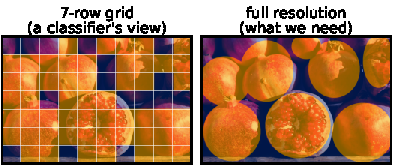
\includegraphics{seg_dilemma.pdf}\par}
    \vskip 6pt
    \fcolorbox{armblue}{armblue!8}{\parbox{0.95\linewidth}{\small
      Two ways out - both computed by hand in [48]:
      \begin{enumerate}\setlength\itemsep{0pt}
        \item \textbf{shrink, then grow back}: transposed convolution (next), U-Net;
        \item \textbf{never shrink}: dilated convolution (after it).
      \end{enumerate}}}
  \end{columns}
\end{frame}

% 2026-10-14 (instructor: "demo transposed conv better"): the TikZ sketch (one stamp, no numbers)
% became a 5-click worked example, py_src/transposed_anim.py (checked against
% torch.nn.functional.conv_transpose2d).
\begin{frame}{Transposed convolution: a learnable way up}
  \small
  Convs and pools \textbf{shrink} maps; a per-pixel answer needs full resolution back. A
  \textbf{transposed convolution} goes up: each input number \textbf{stamps} a scaled copy of
  the kernel onto a bigger output, and overlapping stamps \textbf{add}. \textbf{(Click.)}
  \vskip 2pt
  {\centering
  \only<1>{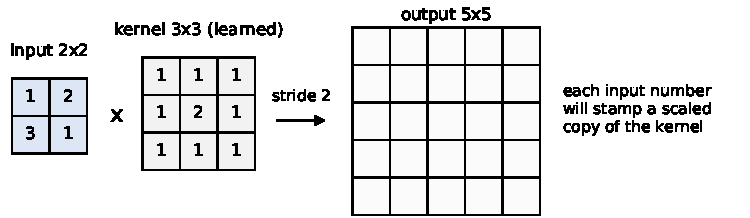
\includegraphics[width=0.82\linewidth]{transposed_anim_0.pdf}}%
  \only<2>{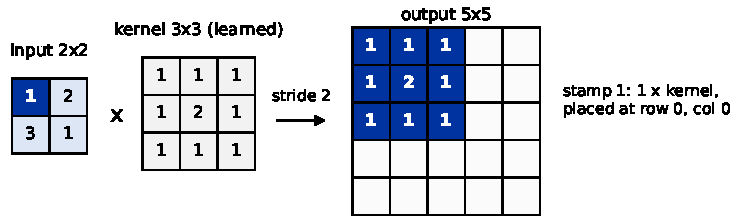
\includegraphics[width=0.82\linewidth]{transposed_anim_1.pdf}}%
  \only<3>{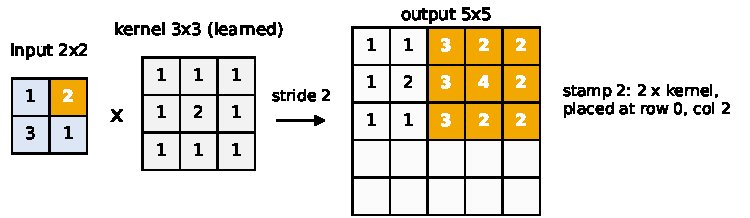
\includegraphics[width=0.82\linewidth]{transposed_anim_2.pdf}}%
  \only<4>{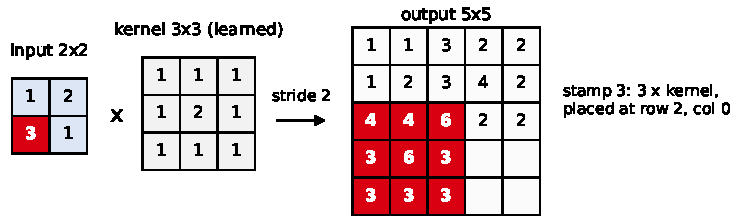
\includegraphics[width=0.82\linewidth]{transposed_anim_3.pdf}}%
  \only<5>{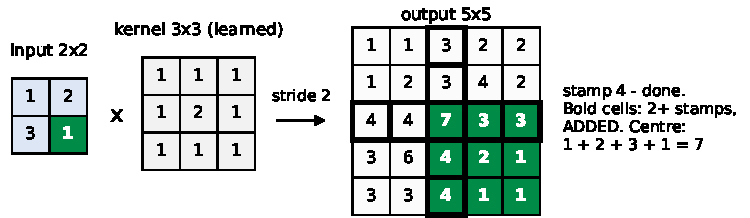
\includegraphics[width=0.82\linewidth]{transposed_anim_4.pdf}}\par}
  \vskip 2pt
  \begin{columns}[T]
    \column{0.5\textwidth}
    \footnotesize
    Output size $(2 - 1)\cdot 2 + 3 = 5$. The 9 kernel numbers are \textbf{learned}. U-Net
    uses a $2\times2$ kernel, stride 2: no overlap, each cell becomes a $2\times2$ block -
    exactly double. (Name: a conv is a matrix multiply $\yv = K\mathbf{z}$; this one uses
    $K^\top$'s pattern to go back up.)
    \column{0.48\textwidth}
    \fcolorbox{armorange}{armorange!12}{\parbox{0.95\linewidth}{\footnotesize
      \textbf{Watch-out: checkerboard.} The bold cells got more stamps; on real images that
      uneven overlap tiles a checker pattern. Fix: kernel divisible by the stride, or
      upsample then convolve
      (\href{https://distill.pub/2016/deconv-checkerboard/}{\color{armblue}\underline{Odena et
      al., 2016}}).}}
  \end{columns}
\end{frame}

\begin{frame}{Dilated convolution: context without losing resolution}
  \begin{columns}[T]
    \column{0.47\textwidth}
    \small
    Insert \textbf{gaps} into the kernel: a $3\times3$ kernel with dilation $d$ taps
    cells $d$ apart. \textbf{(Click to widen.)}
    \vskip 4pt
    \begin{itemize}
      \item Same $9$ weights, wider view - no pooling, no lost pixels.
      \item{} [49] grew the receptive field by \emph{stacking}; dilation grows it
        \textbf{per layer}.
      \item Beyond images: \textbf{WaveNet} audio and temporal convolutional networks
        for time series stack dilated 1D convs.
    \end{itemize}
    \vskip 4pt
    \fcolorbox{armblue}{armblue!8}{\parbox{0.95\linewidth}{\small
      Segmentation's dilemma solved: see the \textbf{whole scene} while keeping
      \textbf{per-pixel} detail.}}
    \column{0.53\textwidth}
    \begin{center}
      \only<1>{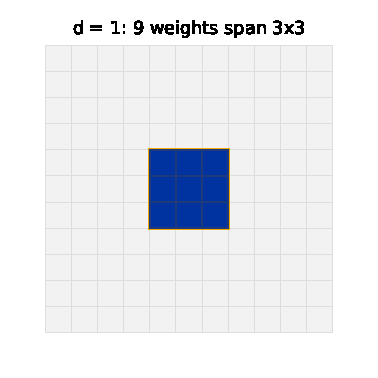
\includegraphics[height=0.64\textheight]{dilation_anim_0.pdf}}%
      \only<2>{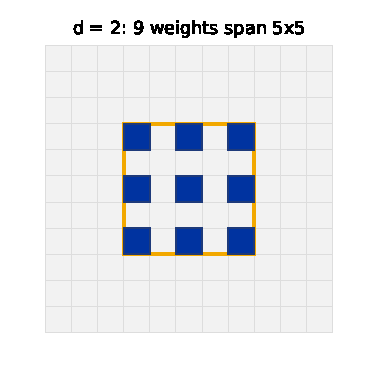
\includegraphics[height=0.64\textheight]{dilation_anim_1.pdf}}%
      \only<3>{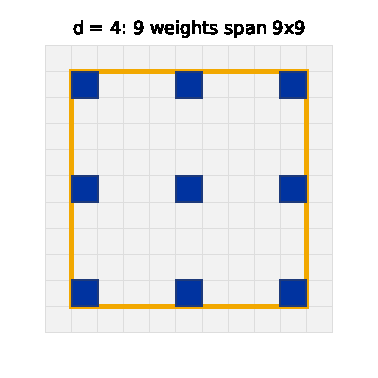
\includegraphics[height=0.64\textheight]{dilation_anim_2.pdf}}%
    \end{center}
  \end{columns}
\end{frame}

\begin{frame}{Stack dilations and the field explodes}
  \begin{center}
    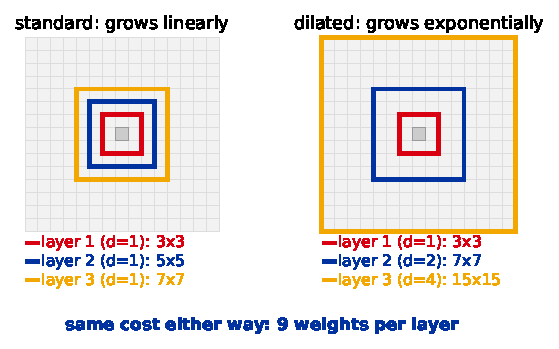
\includegraphics[height=0.68\textheight]{receptive_field_dilated.pdf}
  \end{center}
  \vskip 2pt
  \fcolorbox{armblue}{armblue!8}{\parbox{0.97\linewidth}{\small
      Doubling the dilation each layer ($d = 1, 2, 4$) grows the receptive field
      \textbf{exponentially}: $15 \times 15$ instead of $7 \times 7$, for the same nine
      weights per layer (compare [49]'s receptive-field frame).}}
\end{frame}

% 2026-10-13: the paper's Fig. 1 (unet_paper.png, kept in fig/borrowed/) was unreadable at its
% slot size; replaced by unet_shapes.pdf (py_src/unet_shapes.py), a 3-level padded U-Net on a
% 224x224 photo whose shapes are traced through real torch layers and asserted.
\begin{frame}{U-Net: the segmentation workhorse}
  \vskip -4pt
  {\centering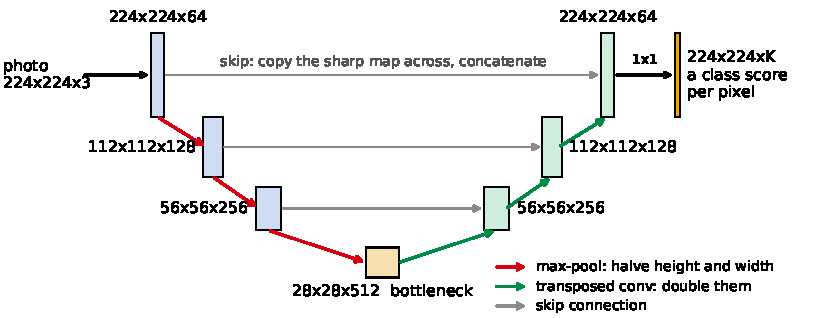
\includegraphics[width=0.93\linewidth]{unet_shapes.pdf}\par}
  \vskip 2pt
  \begin{columns}[T]
    \column{0.52\textwidth}
    \small
    \textbf{Down}: pooling trades resolution for context ($224 \to 28$). \textbf{Up}:
    transposed convs climb back to $224$. \textbf{Skips}: the sharp early maps are
    \emph{concatenated} onto the upsampled ones - the detail the bottleneck lost.
    \column{0.46\textwidth}
    \fcolorbox{armblue}{armblue!8}{\parbox{0.95\linewidth}{\small
      [49]'s skips again - there they rescued \textbf{optimization}, here they carry
      \textbf{resolution}.}}
    \vskip 1pt
    {\scriptsize\color{gray} Ronneberger et al., 2015 (medical images; four levels deep).}
  \end{columns}
\end{frame}

% 2026-10-14 (instructor: "I don't get what's the input, what's the output"): the LMU 2x2 grid had
% the input in the bottom-right corner; road_panels.py re-lays the same four panels in reading
% order with explicit IN / OUT titles.
\begin{frame}{U-Net in action: roads from the sky}
  {\centering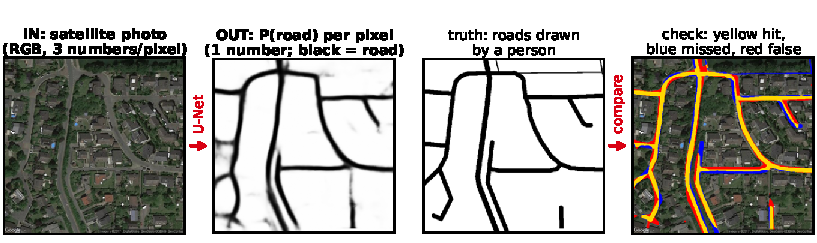
\includegraphics[width=0.9\linewidth]{road_panels.pdf}\par}
  {\raggedleft\scriptsize\color{gray} LMU I2DL, CC BY 4.0, rearranged.\par}
  \vskip 2pt
  \noindent\begin{minipage}[t]{0.52\linewidth}
    \small
    \textbf{In:} a satellite tile, $512\times512\times3$ - a colour photo. \textbf{Out:}
    \textbf{one number per pixel}, $512\times512\times1$: "this pixel is road", as a
    probability. Loss: [11]'s log-loss, once per pixel, summed.
  \end{minipage}\hfill
  \begin{minipage}[t]{0.46\linewidth}
    \vspace{0pt}\fcolorbox{paramgreen}{paramgreen!8}{\parbox[t]{0.95\linewidth}{\small
      Same size in, same size out - only the channels change ($3 \to 1$). The check panel is
      [12]'s confusion matrix, \emph{painted onto the map}.}}
  \end{minipage}
\end{frame}

% ================================================================
% 2026-10-14 (instructor: "spend a couple of slides on industry standards nowadays, like SAM").
% Reopens the July interview's "no SAM screenshot" only partly: the SAM frame uses a self-drawn
% diagram (sam_diagram.py), not a screenshot. Facts: Kirillov et al., arXiv 2304.02643 (Apr 2023):
% "Given a precomputed image embedding, the prompt encoder and mask decoder run in a web browser,
% on CPU, in 50ms"; SA-1B = 11M images, 1.1B masks, final stage fully automatic. SAM 2: Meta,
% 2024-07-29, images and video. SAM 3: Meta, 2025-11-19/20, text or exemplar prompts, every
% instance (arXiv 2511.16719). YOLO26: Ultralytics, Jan 2026 (NMS-free). YOLO27: announced
% 2026-09-13, docs say "not yet available" (checked 2026-10-14). RF-DETR: Roboflow, arXiv
% 2511.09554, ICLR 2026, Apache 2.0. Gemini returns boxes as box_2d (ai.google.dev, checked
% 2026-10-14).
\section{The 2026 toolbox}

\begin{frame}[plain]
  \vfill
  \begin{center}
    {\Large\color{popblue}\textbf{What people actually use in 2026}}\\[0.9em]
    \begin{minipage}{0.82\textwidth}\centering\small
      Almost nobody trains a detector or a segmenter from scratch now. They start from a few
      big pretrained models - and one family made "segment this" a single click.
    \end{minipage}
  \end{center}
  \vfill
\end{frame}

\begin{frame}{Segment Anything: one model, any object}
  \vskip -2pt
  {\centering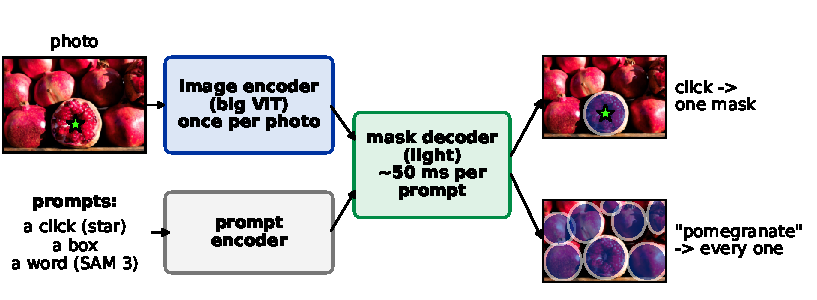
\includegraphics[width=0.8\linewidth]{sam_diagram.pdf}\par}
  \vskip 1pt
  \begin{columns}[T]
    \column{0.5\textwidth}
    \footnotesize
    \textbf{SAM} (Meta, 2023): click or draw a box, get a mask - even for objects it never
    saw. The heavy encoder runs \textbf{once} per photo; each prompt costs only the light
    decoder, \textbf{$\sim$50 ms on a CPU}: it feels instant. Its 1.1 billion training masks
    were drafted by SAM and fixed by people ([50]).
    \column{0.48\textwidth}
    \footnotesize
    \textbf{SAM 2} (2024): video - click once, the mask follows the object.
    \vskip 2pt
    \textbf{SAM 3} (Nov 2025): type "pomegranate", get a mask for \textbf{every} one -
    detection and segmentation by prompt.
    \vskip 2pt
    {\scriptsize\color{gray} Masks in the diagram drawn by hand, not by SAM.}
  \end{columns}
\end{frame}

\begin{frame}{The 2026 toolbox}
  \small
  \begin{center}
    \begin{tabular}{>{\raggedright\arraybackslash}p{3.4cm} >{\raggedright\arraybackslash}p{5.1cm}
                    >{\raggedright\arraybackslash}p{3.2cm}}
      \textbf{You need ...} & \textbf{Reach for} & \textbf{You provide}\\
      \hline
      boxes for \emph{your} classes, fast, on a small device & Ultralytics YOLO (YOLO26, Jan
        2026); RF-DETR (Roboflow, 2025) & labeled boxes - fine-tune ([50])\\[3pt]
      boxes for anything you can name & open-vocabulary detectors: YOLO-World, Grounding DINO
        & class names as text\\[3pt]
      masks & SAM 2 (click or box, also video); SAM 3 (a typed concept) & a prompt\\[3pt]
      features for a new task & DINOv3, frozen ([50]) & a linear head\\[3pt]
      an answer in words - or boxes for a question & vision-language models (Gemini, Qwen-VL
        return boxes as text) & a question\\
    \end{tabular}
  \end{center}
  \vskip 4pt
  \fcolorbox{paramgreen}{paramgreen!8}{\parbox{0.97\linewidth}{\small
    The pattern: big promptable models draft labels and build prototypes; a small fine-tuned
    model runs on the belt. Lists like this age fast - YOLO27 was announced in September 2026
    and is not out yet. Check before you trust any "latest", including this one.}}
\end{frame}

% ================================================================
\section{The sorting line, completed - and the chapter close}

\begin{frame}[plain]
  \vfill
  \begin{center}
    {\Large\color{popblue}\textbf{The sorting line, completed}}\\[0.9em]
    \begin{minipage}{0.82\textwidth}\centering\small
      Cash in the running example - then zoom out on the whole chapter.
    \end{minipage}
  \end{center}
  \vfill
\end{frame}

\begin{frame}{One scenario, four output structures}
  The pomegranate line, end to end:
  \vskip 4pt
  \begin{center}\small
    \begin{tabular}{l l l}
      \textbf{Question on the line} & \textbf{Task} & \textbf{Tool}\\
      \hline
      "what grade is this fruit?" & classification & [49]'s ResNet-18, fine-tuned in [50]\\
      "is it grading fruit or belt?" & attribution & [50]'s Grad-CAM audit\\
      "how many fruit, and where?" & detection & a fine-tuned YOLO\\
      "where exactly is the bruise?" & segmentation & a small U-Net for the cutter\\
    \end{tabular}
  \end{center}
  \vskip 6pt
  Swap the nouns and it is the same story everywhere: roads on satellite tiles, tumors
  on MRI slices, cracks on factory parts.
  \vskip 4pt
  \fcolorbox{paramgreen}{paramgreen!8}{\parbox{0.97\linewidth}{\small
      One backbone vocabulary - conv, pool, skip, upsample - and the \textbf{output
      structure} turns it into whichever tool the problem needs.}}
\end{frame}

% 2026-10-13 addition: generalizes the deck's thesis past the four zoo tasks. MediaPipe Hands:
% palm detector, then a landmark model that regresses 21 3D hand-knuckle coordinates
% (google-ai-edge/mediapipe docs/solutions/hands.md; ai.google.dev hand_landmarker guide,
% checked 2026-10-13).
\begin{frame}{More output structures, same backbone}
  The task zoo had four outputs. Swap the head again and you get more:
  \vskip 4pt
  \begin{itemize}\setlength\itemsep{4pt}
    \item \textbf{Keypoints} - a fixed list of points per object. Google's MediaPipe hand
      model first \emph{detects} the hand, then regresses \textbf{21 points} on it
      (knuckles, fingertips): $21 \times 3 = 63$ numbers, [01]'s regression. Gesture Snake's
      thumb direction could be a rule on two of those points.
    \item \textbf{Depth} - a \emph{number} per pixel instead of a class: a U-Net-shaped
      network with a regression loss.
    \item \textbf{Text} - a caption, or an answer about the photo: a vision backbone feeding a
      language model (vision-language models, later in the course).
  \end{itemize}
  \vskip 6pt
  \fcolorbox{armblue}{armblue!8}{\parbox{0.97\linewidth}{\small
    Detection = classification + regression in slots. Segmentation = classification per
    pixel. Keypoints = regression on a fixed list. Depth = regression per pixel.
    \textbf{Pick the output - the loss follows.}}}
\end{frame}

% 2026-10-14 (instructor: "remove the movie review thing on the right, it's confusing"):
% text_1d_conv.png is no longer embedded (the file stays in fig/borrowed/).
\begin{frame}{Same idea, other shapes: 1D and 3D}
  Nothing about convolution says "image". The window slides over whatever grid the data lives
  on:
  \vskip 6pt
  \begin{itemize}\setlength\itemsep{4pt}
    \item \textbf{1D} - sequences: accelerometer traces for activity recognition, audio.
      [48] \emph{opened} with a 1D kernel sliding over a sequence - that was the real thing,
      not a warm-up.
    \item \textbf{2D} - images: this whole chapter.
    \item \textbf{3D} - volumes: video (stacked frames), MRI and CT scans - the kernel slides
      in $x$, $y$ \emph{and} $z$.
  \end{itemize}
  \vskip 8pt
  \fcolorbox{armblue}{armblue!8}{\parbox{0.97\linewidth}{\small
      Convolution is a \textbf{structural prior} - "nearby means related, patterns repeat" -
      not an image trick. Wherever that assumption holds, the same layer works.}}
\end{frame}

% 2026-10-14 (instructor: "spend a couple of slides explaining neural style transfer, idea-wise").
% The old one-frame showcase split: two style-transfer frames (style_transfer_figs.py; Gatys et al.,
% arXiv 1508.06576, Methods: VGG-19's 16 conv + 5 pooling layers, content conv4_2, style
% conv1_1..conv5_1, gradient descent from a white-noise image, style = Gram matrix of filter
% responses) + the GAN frame. Johnson, Alahi & Fei-Fei, "Perceptual Losses for Real-Time Style
% Transfer and Super-Resolution", ECCV 2016.
\begin{frame}{CNNs can also paint: neural style transfer}
  \small
  One more output structure: a \textbf{whole new picture}. Gatys et al.\ (2015) repainted a
  photo in Van Gogh's style with a network that was only ever trained to \emph{classify}.
  \vskip 2pt
  {\centering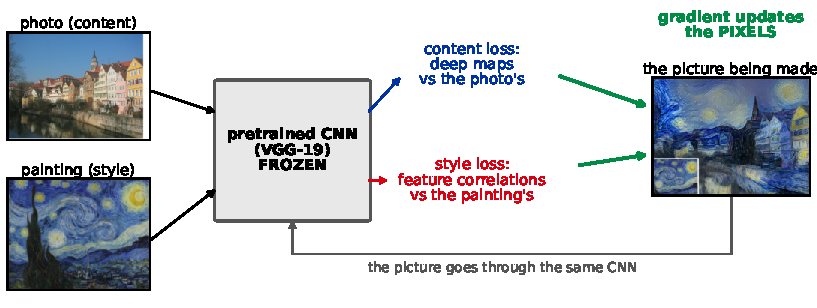
\includegraphics[width=0.86\linewidth]{style_loop.pdf}\par}
  \vskip 2pt
  \fcolorbox{armblue}{armblue!8}{\parbox{0.97\linewidth}{\small
    Nothing gets trained except the \textbf{picture}. Start from noise, run it through the
    frozen VGG-19 ([49]), measure two losses, and let gradient descent change its
    \textbf{pixels} - the same backprop as training, with the image as the parameter.}}
\end{frame}

\begin{frame}{What "style" means to a CNN}
  \small
  \textbf{Content:} the photo's deep-layer maps - they keep \emph{what is where} (the layout),
  not exact pixels ([50]'s feature hierarchy). \textbf{Style:} for each layer, count which
  features fire \emph{together} - the \textbf{Gram matrix}
  $G_{ij} = \sum_{\text{positions } p} F_i(p)\, F_j(p)$:
  \vskip 2pt
  {\centering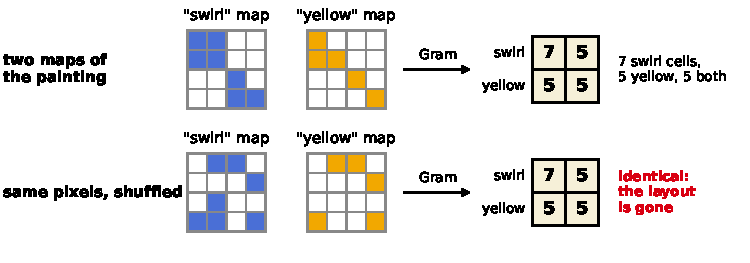
\includegraphics[width=0.84\linewidth]{gram_toy.pdf}\par}
  \vskip 2pt
  \begin{columns}[T]
    \column{0.5\textwidth}
    \footnotesize
    Summing over positions throws away \emph{where} - the move [49]'s global average pooling
    made. What survives: which colours, textures and strokes go together. A fair definition of
    style.
    \column{0.48\textwidth}
    \fcolorbox{paramgreen}{paramgreen!8}{\parbox{0.95\linewidth}{\footnotesize
      Weight the two losses: more style, more painting. Since 2016 a network is
      \emph{trained} to do it in one pass (Johnson et al.) - the real-time photo filters.}}
  \end{columns}
\end{frame}

\begin{frame}{CNNs can also invent: GANs}
  \begin{columns}[T]
    \column{0.5\textwidth}
    \begin{center}
      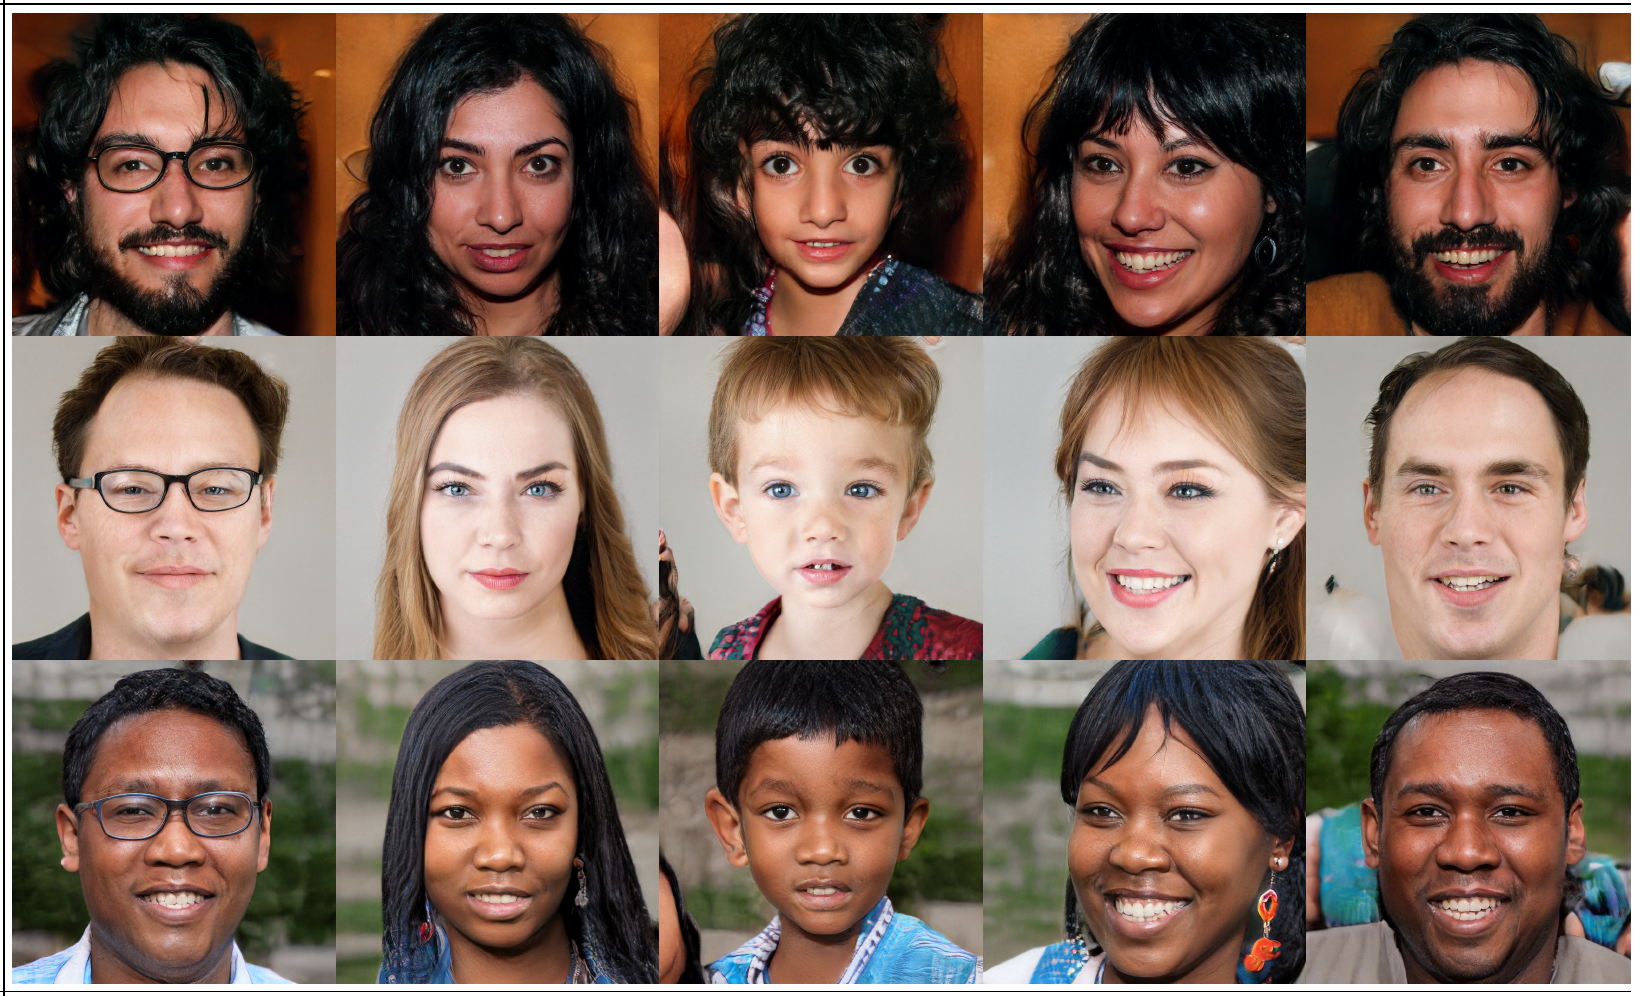
\includegraphics[width=\linewidth]{stylegan_faces.png}\\[1pt]
      {\scriptsize None of these people exist (StyleGAN, Karras et al. 2019).}
    \end{center}
    \column{0.48\textwidth}
    \small
    \textbf{GANs}: two networks duel - a generator forges images, a discriminator calls
    fakes, both improve until the fakes pass (Goodfellow et al. 2014).
    \vskip 4pt
    The generator upsamples noise into pixels with \textbf{transposed convolutions} - the
    stamps from the segmentation section.
    \vskip 6pt
    \fcolorbox{armblue}{armblue!8}{\parbox{0.95\linewidth}{\small
      Honest footnote: for image \emph{generation}, \textbf{diffusion} has largely taken over
      ([49] epilogue) - GANs live on in upscaling and faces. Mechanics belong to the diffusion
      chapter (L27-L31).}}
  \end{columns}
\end{frame}

\begin{frame}{The inductive-bias ledger}
  What this chapter really bought us - stated honestly:
  \vskip 6pt
  \begin{itemize}
    \item CNNs \textbf{assume} locality and translation equivariance ([48]'s two wishes:
      "nearby means related, a detector useful here is useful there").
    \item When the assumption is \emph{true} - images, audio, volumes - it acts as
      \textbf{regularization by architecture}: win with \emph{less data}.
    \item When it is \emph{false}, it costs you: \textbf{tabular data} still belongs to
      trees and boosting (ch4, and [40]'s tabular caveat), and images where
      \textbf{global context} dominates strain the local prior.
  \end{itemize}
  \vskip 8pt
  \fcolorbox{armblue}{armblue!8}{\parbox{0.97\linewidth}{
      There is no universally best architecture - only assumptions that \textbf{match or
      mismatch} the data. Choosing the bias \emph{is} the modeling decision.}}
\end{frame}

\begin{frame}{The chapter in one strip}
  \begin{center}
    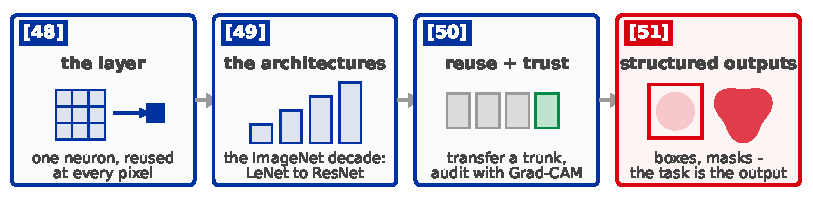
\includegraphics[width=0.99\linewidth]{chapter_arc.pdf}
  \end{center}
  \vskip 6pt
  \begin{center}\small
    One layer $\to$ architectures $\to$ reuse and trust $\to$ structured outputs.\\
    You can now read, adapt, audit and deploy the networks that do most of the world's
    looking.
  \end{center}
\end{frame}

\begin{frame}{Hand-off: Vision Transformers}
  The [49] epilogue's loose thread, tied:
  \vskip 6pt
  \begin{itemize}
    \item \textbf{ViT} cuts the image into patches and feeds them to a transformer as a
      \emph{sequence} - \textbf{no convolution at all} (Dosovitskiy et al., 2021).
    \item It \textbf{drops the convolutional prior} - and buys it back with
      \textbf{scale}: with enough pretraining data, attention \emph{learns} locality
      instead of assuming it.
    \item Small data? The CNN prior still wins. Web-scale data? Attention takes the
      frontier. The ledger from two slides ago, live in 2026.
  \end{itemize}
  \vskip 8pt
  \fcolorbox{paramgreen}{paramgreen!8}{\parbox{0.97\linewidth}{\small
      Attention, transformers and the GenAI stack get their own chapters - and the road
      there runs through RNNs, next.}}
\end{frame}

% ================================================================
\section*{Recap}

\begin{frame}{Recap}
  \begin{itemize}
    \item The \textbf{output structure defines the task}: label $\to$ box $\to$ box per
      object $\to$ class per pixel.
    \item Detection $=$ many \textbf{slots}, each a box $+$ a \textbf{confidence} (predicted
      $c_o$): anchors at every grid cell, shifted and stretched by a head, in one pass. Then
      \textbf{IoU}, \textbf{NMS}, \textbf{mAP} ($=$ [12] over boxes).
    \item \textbf{YOLO}: the centre's cell reports the object, computed from the whole photo;
      loss $=$ box regression $+$ confidence $+$ class, added. \textbf{Label every object}.
    \item \textbf{Separable convs} make it fit on a belt camera ($\sim$23$\times$ cheaper).
    \item Segmentation: \textbf{U-Net} $=$ down, up (\textbf{transposed convs}: stamps that
      add), skips; \textbf{dilation} for context. 2026: \textbf{SAM} masks on a click or a word.
    \item Convolution is a \textbf{prior with a domain} - and it can paint: style $=$ the
      \textbf{Gram matrix}, which features fire together.
  \end{itemize}
  \vskip 6pt
  \fcolorbox{paramgreen}{paramgreen!8}{\parbox{0.97\linewidth}{
      \textbf{Next:} the Gesture Snake practical - train a CNN on \emph{your} webcam
      photos, audit it with Grad-CAM, and play with it. Then a new chapter: networks with
      \textbf{memory} - RNNs (L20).}}
\end{frame}

\end{document}

% ================================================================
% Provenance:
%   Deck: L19 Vision Tasks - Detection and Segmentation (12_cnn, chapter closer).
%   Built 2026-07-14 from 51_vision_tasks_OUTLINE.md (approved; interview-locked
%   2026-07-13, GANs/style-transfer showcase added 2026-07-14) + CNN_CHAPTER_PLAN.md.
%
%   Sources consulted (REDERIVE, read-only): LMU I2DL cnn2/{dilated-transposed,
%   separable-convolutions-flattening, convolution-types}.tex, cnn1/application.tex
%   (label-vector trick, task-zoo idea), cnn3/modern-cnn-2.tex (U-Net). Detection
%   vocabulary (IoU/NMS/mAP, families, YOLO grid) authored from the outline - no LMU
%   upstream. Credit line on title frame per chapter policy (CC BY 4.0).
%
%   Verified numbers (asserted in the figure scripts before typesetting):
%   - IoU worked example: A=(0,0)-(4,4), B=(2,0)-(6,4) -> inter 8, union 24, IoU 1/3
%     (iou_nms.py).
%   - Separable count: 12x12x3 input, 5x5, 256 out -> standard 256*75*64 = 1,228,800;
%     depthwise 3*25*64 = 4,800 + pointwise 256*3*64 = 49,152 = 53,952; ratio 22.8x,
%     stated as ~23x (separable_count.py).
%   - Dilated RF: stacked d=1,2,4 -> 3, 7, 15 vs standard 3, 5, 7
%     (receptive_field_dilated.py).
%   - YOLO v1 facts (Redmon et al. 2016): 7x7 grid, 2 boxes/cell, per-cell class
%     probabilities, 98 boxes, 7x7x30 output tensor (B*5+C with C=20), one pass.
%
%   Figures (py_src -> fig, ma venv): task_zoo.py (task_zoo.pdf - 4 overlays,
%   hand-placed coords on the web photo, semantic tint baked into RGB per LEARNINGS);
%   iou_nms.py (iou_nms.pdf + iou_only.pdf + nms_only.pdf; boxes/NMS logic shared);
%   nms_anim.py (nms_anim_0..4.pdf, 5-frame mandatory ANIM; imports iou_nms so the
%   final frame equals the static right panel); chapter_arc.py (chapter_arc.pdf,
%   ribbon-style 4-beat strip, L19 hot in red); receptive_field_dilated.py
%   (receptive_field_dilated.pdf + dilation_anim_0..2.pdf - NEW files; L17's
%   receptive_field.pdf deliberately NOT regenerated); separable_count.py
%   (separable_count.pdf, labeled bars).
%
%   Borrowed (fig/borrowed/): pomegranate_market.jpg (WEB-IMG, Wikimedia Commons
%   "Pomegranates at farmers market (43134440935).jpg", 1920x1280 - the interview-
%   locked multi-fruit stall shot); yolo_grid.png (YOLO paper Fig 2, arXiv:1506.02640,
%   300dpi crop); unet_paper.png (U-Net paper Fig 1, arXiv:1505.04597);
%   maskrcnn_framework.png (Mask R-CNN paper Fig 1, arXiv:1703.06870);
%   gatys_content.png + gatys_starry.png (Gatys et al. Fig 2 panels A and C,
%   arXiv:1508.06576); stylegan_faces.png (StyleGAN paper Fig 3 crop, all-generated
%   faces, arXiv:1812.04948). COPY-IMG (whitelisted): unet_road_result.png = LMU
%   lecture_i2dl cnn3/plots/outlook/31.png, attribution line on the frame (CC BY 4.0);
%   text_1d_conv.png = cropped from LMU I2DL week24 01_convolution-types.pdf p12
%   (char-level text as a 1D signal), embedded on the "Same idea, other shapes: 1D and
%   3D" frame to give that prior-not-an-image-trick claim a concrete figure; no
%   per-image credit line (chapter-level LMU credit on the title frame, per instructor).
%
%   Key decisions (details in 51_DECISIONS.md): conv variants just-in-time per the
%   interview (separable in detection, transposed+dilated in segmentation, 1D/3D in
%   the close); IoU presented not computed; mAP got its own short frame; separable
%   split into idea+count; dilated split into kernel-anim + stacked-RF frames; U-Net
%   split into architecture + road-result frames; GANs/style-transfer stayed ONE
%   frame (3-image strip). Interview-rejected items honored: no real YOLO outputs,
%   no SAM screenshot, no Dice line, no transfer-learning re-teach.
%
%   2026-07-21 addition: one-line disambiguation on "Separable convolutions: the idea" -
%   distinguishes SPATIALLY separable (2D kernel -> two 1D passes, Sobel, L16) from the
%   DEPTHWISE separable taught here (naming-gap fix from the conv-type coverage check).
%
%   2026-09-22 pre-delivery pass (instructor away - autonomous): L11/L12 -> [11]/[12]
%   (same decks, current numbering); "L14's honest-scope frame" -> [40]'s tabular caveat
%   (LMU 01_introduction, embedded in [40]); the ledger's "translation equivariance" now
%   points back to L16's two wishes, which define it since the 2026-09-22 L16 pass. NMS frame
%   gained a 2026 footnote: DETR (Carion et al., ECCV 2020, set prediction, no NMS) and
%   Ultralytics YOLO26 (released January 2026, NMS-free by default). Web-verified 2026-09-22.
%
%   Same day, after a Sonnet student review of the rendered deck: NEW "mAP by hand" (one
%   class, 2 truths, ranked TP/FP/TP/FP -> P 1/.5/.67/.5, R .5/.5/1/1, AP .83; reversed
%   ranking -> AP .5) and NEW "Decoding one YOLO cell, by hand" (448 px / 7 = 64 px cells;
%   cell (3, 2) with x=.5, y=.25, w=.2, h=.3, conf .8, P(class|obj) .9 -> centre (160, 208),
%   90 x 134 px, score .72; "responsible" predictor = highest IoU, from the paper). The
%   transposed-conv watch-out now points at L16's 1D stamp toy for WHY the checkerboard
%   appears. Reviewer-proposed cuts (GAN/style-transfer frame, 1D/3D frame) NOT applied:
%   both were instructor-requested in the 2026-07-13/14 interviews.
%
%   2026-09-30 error fixes (folder now ml/12_cnn): mAP-by-hand reversed ranking said AP .5,
%   which is the INTERPOLATED value - the slide's own rule gives .5/3 + .5/2 = .42 (sklearn
%   average_precision_score = 0.4167), now stated; sorting-line table said "L16's CNN, built
%   via L18 transfer" (L18 fine-tunes L17's ResNet-18); ViT hand-off said "we follow it there
%   next" while the Next box says RNNs come next; recap "L12" -> [12].
%
%   2026-10-01 pass (instructor request "improve slides"): HW4 (YOLO + NMS knob + dilated
%   swap) was never built. The NMS frame now says what the threshold does instead of "you
%   will turn this knob in HW4"; the Next box points to the Gesture Snake practical
%   (DECISIONS #58). SSD and TCN spelled out (TCN as words). chapter_arc.py: the four panels
%   ran 0.04 past the axes (0.12 + 4*2.86 + 3*0.36 = 12.64 > 12.6), cutting off the L19
%   panel's right edge - start/gap tightened, figure regenerated.
%
%   2026-10-01 rounds 2-3 (instructor review): every figure redrawn at its slot size
%   (detect_small_figure_text.py: 12 pages under 5.5 pt on the committed PDF -> 0); the NMS
%   frame went to two columns so the animation is readable; task zoo embedded by height;
%   separable_count lost its side note (the arrow ran through it; the split is in the
%   equations). SAM box updated to SAM 3 (Meta, 2025: text-prompted, every instance), as in
%   the L17 epilogue. Checkerboard watch-out links Odena et al.'s Distill article.
%
%   2026-10-02 (instructor): (1) NEW "Why a detector answers with so many boxes" before IoU,
%   built on a REAL detector run (detector_candidates.py: torchvision SSDlite320-MobileNetV3,
%   COCO weights, results cached in results/detector_candidates.npz/.json): 3,234 candidates
%   per photo, 401 (box, class) pairs > 5%, 45 above 0.4, 7 after class-agnostic NMS at 0.45 -
%   six fruit called "apple"/"orange" plus one box around the whole crate. (2) NEW
%   "Segmentation's dilemma: see far, stay sharp" before transposed conv (seg_dilemma.py, the
%   task-zoo mask on a 7-row grid vs full resolution): says why transposed and dilated conv
%   appear here - shrink-then-grow-back vs never-shrink.
%
%   2026-10-13 pedagogy + gaps pass (instructor: "improve them pedagogically, find important
%   gaps"); details in 51_DECISIONS.md #13-#18:
%   - FIX: the cold open's answer said the [51] classifier outputs "pomegranate"; it outputs a
%     GRADE (export/market/juice), so it grades the whole stall as one fruit.
%   - Label-vector frame: c_o = 0 -> the rest is "don't care" (sets up detector training).
%   - NEW "Training the grid: who learns what" (yolo_targets.py on the belt photo, counts
%     asserted): centre-cell rule, 8 responsible of 98, 90 pushed to confidence 0, the
%     imbalance ([12]) and YOLO's lambda_noobj 0.5 / lambda_coord 5, focal loss.
%   - NEW "Your own detector: label boxes, or prompt for them": Ultralytics data guidance,
%     "label every object" (an unlabeled fruit becomes a 'nothing here' target), YOLO-World,
%     SAM 3, draft-then-correct. Cashes [51]'s "boxes cost money" thread.
%   - U-Net frame: the paper figure (unreadable at slot size) replaced by unet_shapes.pdf,
%     a 3-level padded U-Net with traced, asserted shapes; unet_paper.png stays in borrowed/.
%   - NEW "More output structures, same backbone": keypoints (MediaPipe's 21 hand points),
%     depth per pixel, text; "pick the output, the loss follows".
%   - chapter_arc.pdf badges L16-L19 -> [48], [50], [51], [52]; recap trimmed and extended.
%
%   Forward pointer: the Gesture Snake practical (ml/12_cnn/gesture_snake/); next chapter
%   ch7_rnn L20 RNN Foundations.
%
%   2026-10-14 instructor review (13 requests + "add the yolos founders cv"), 36 -> 49 frames,
%   details in 51_DECISIONS.md #19-#31; every new frame carries a dated comment with its
%   sources. New: "'Nothing here' has to be an answer"; three candidate-box frames from a real
%   run (candidate_boxes.py: crop-and-classify, SSDlite's per-cell heads, anchors + offsets);
%   section "Building a detector" + transition; "Meet YOLO's author" (redmon_resume.png); "A
%   cell is an address, not a window" (yolo_cell_figs.py); "The detection loss: regression and
%   classification, added"; "Making it fast: separable convolutions" (separable_idea.py);
%   transposed conv as a 5-click animation (transposed_anim.py); roads re-laid out IN -> OUT
%   (road_panels.py); section "The 2026 toolbox" (sam_diagram.py + a table); style transfer
%   pair (style_transfer_figs.py). Removed: the movie-review figure on the 1D/3D frame.
%   Recap rewritten.
%
%   2026-10-15: renumbered to the playlist after delivery (instructor: no practical between
%   [48] and transfer learning): [50] -> [49], [51] -> [50], [52] -> [51], the practical
%   [53] -> [52]; deck files renamed to match. Slide text uses the new labels; labels written in
%   this block before this date keep the old ones.
